\documentclass{sig-alternate-05-2015}
\graphicspath{{images/}}
\DeclareGraphicsExtensions{.eps}
\usepackage{subcaption}
\usepackage{tabularx}
\usepackage{multirow}

\hyphenation{de-term-in-a-tion self-de-term-in-a-tion}

\begin{document}

% Copyright
\setcopyright{acmcopyright}

% DOI
\doi{10.475/123_4}

% ISBN
\isbn{123-4567-24-567/08/06}

%Conference
\conferenceinfo{ITiCSE '16}{July 11--13, 2016, Arequipa, Peru}

\acmPrice{\$15.00}

\title{Game Development for Computer Science Education}

\numberofauthors{6}
\author{
\alignauthor
Chris Johnson\\
       \affaddr{University of Wisconsin, Eau Claire}\\
       \email{johnch@uwec.edu}
\alignauthor
Monica McGill\\
       \affaddr{Bradley University}\\
       \email{mmcgill@bradley.edu}
\alignauthor
Durell Bouchard\\
       \affaddr{Roanoke College}\\
       \email{bouchard@roanoke.edu}
\and
\alignauthor
Michael K. Bradshaw\\
       \affaddr{Centre College}\\
       \email{michael.bradshaw@\\centre.edu}
\alignauthor
V\'{i}ctor A. Bucheli\\
       \affaddr{Universidad del Valle}\\
       \email{victor.bucheli@\\correounivalle.edu.co}
\alignauthor
Laurence D. Merkle\\
       \affaddr{Air Force Institute of Technology}\\
       \email{laurence.merkle@afit.edu}
\and
\alignauthor
Michael James Scott\\
       \affaddr{Falmouth University}\\
       \email{michael.scott@falmouth.ac.uk}
\alignauthor
Z Sweedyk\\
       \affaddr{Harvey Mudd College}\\
       \email{z@cs.hmc.edu}
\alignauthor
J. \'{A}ngel Vel\'{a}zquez-Iturbide\\
       \affaddr{Universidad Rey Juan Carlos}\\
       \email{angel.velazquez@urjc.es}
\and
\alignauthor
Zhiping Xiao\\
       \affaddr{University of California at Berkeley}\\
       \email{patricia.xiao@berkeley.edu}
\alignauthor
Ming Zhang\\
       \affaddr{Peking University}\\
       \email{mzhang\_cs@pku.edu.cn}
}
\date{15 September 2016}

\maketitle
% The code below should be generated by the tool at
% http://dl.acm.org/ccs.cfm
% Please copy and paste the code instead of the example below. 
%
% \begin{CCSXML}
% <ccs2012>
% <concept>
% <concept_id>10010405.10010489</concept_id>
% <concept_desc>Applied computing~Education</concept_desc>
% <concept_significance>500</concept_significance>
% </concept>
% <concept>
% <concept_id>10010405.10010489.10010491</concept_id>
% <concept_desc>Applied computing~Interactive learning environments</concept_desc>
% <concept_significance>500</concept_significance>
% </concept>
% <concept>
% <concept_id>10003120.10003145</concept_id>
% <concept_desc>Human-centered computing~Visualization</concept_desc>
% <concept_significance>300</concept_significance>
% </concept>
% </ccs2012>
% \end{CCSXML}

% \ccsdesc[500]{Applied computing~Education}
% \ccsdesc[500]{Applied computing~Interactive learning environments}

% \printccsdesc

% \keywords{3D printing; Logo; making}
\begin{abstract}




Games can be a valuable tool for enriching computer science education, since they can facilitate a number of conditions that promote learning: student motivation, active learning, adaptivity, collaboration, and simulation. Additionally, they provide the instructor the ability to collect learning metrics with relative ease. As part of 21st Annual Conference on Innovation and Technology in Computer Science Education (ITiCSE 2016), the Game Development for Computer Science Education working group convened to examine the current role games play in computer science (CS) education, including where and how they fit into CS education. Based on reviews of literature, academic research, professional practice, and a comprehensive list of games for computing education, we present this working group report. This report provides a summary of existing digital games designed to enrich computing education, an index of where these games may fit into a teaching paradigm using the ACM/IEEE Computer Science Curricula 2013~\cite{acm13computing}, and a guide to developing digital games designed to teach knowledge, skills, and attitudes related to computer science.





{\em }



\end{abstract}










\section{Introduction}


As part of ITiCSE 2016, the Game Development for Computer Science Education working group convened to examine the current role games play in computer science (CS) education, including where and how they fit into CS education. To guide our discussions and analysis, we began with the following question: in what ways can games be a valuable tool for enriching computer science education?



In our work performed prior to our first face-to-face meeting, we reviewed over 120 games designed to teach computing concepts (which is available for separate download~\cite{appendix}) and reviewed several dozen papers related to game-based learning (GBL) for computing. Hainey~\cite{hainey2010using} found that there is ``a dearth of empirical evidence in the fields of computer science, software engineering and information systems to support the use of GBL.'' This is not unique to CS, however. A review by Papastergiou~\cite{papastergiou2009digital} found limited evidence to support games for learning, and a systematic review by Graafland et al.~\cite{graafland2012systematic} also found no empirically validated games to support education in the medical field.



Though our reviews were not designed to be comprehensive, our findings support these claims. This lack of evidence prevented us from identifying which of these games are most effective in meeting educational outcomes, because little evidence exists to make such claims, and it further prevented us from stating which game design frameworks for CS education might be most effective across various demographics. This required us to rethink our approach and to consider how we would analyze the games and the relevant research in a way that would provide significant value for the broader computer science educational research community. 



The purpose of this working group report, therefore, is: 

\begin{enumerate}
\setcounter{enumi}{0}
\item to provide a summary of existing digital games designed to enrich computing education and an index of where these games may fit into a teaching paradigm using the ACM/IEEE Computer Science Curricula 2013 (CS2013), and 
\item to provide a guide to developing digital games designed to teach knowledge, skills, and/or attitudes related to computer science.
\end{enumerate}




To narrow the broad scope of games, we have chosen to focus on digital games; however, we note that analog games (board games, card games, etc.) can also be an important tool in enriching student learning. Games like those presented in CS Unplugged~\cite{bell2009computer} provide a meaningful way of implementing active learning within a curriculum~\cite{brc12}.



Though an initial goal for this report was to also include a guide for evaluating the effectiveness of games for CS education, given the expansiveness of such a task, we will focus on evaluation and assessment in follow-up work.



Game developers, educational theorists, and others may find value within this report. However, the primary target audience is academic researchers interested in developing games for enriching CS education. This perspective is reflected throughout this report. 



This working group is unconventional in that its work will span two ITiCSE conferences. This first report is divided into several sections, starting with a background that introduces important vocabulary related to game design theory, provides a summary of previous related computer science education research, and provides a summary of relevant educational psychology. It also provides a brief review of games created for computer science education and how these map to CS2013. 



This is followed with case studies of four games designed to teach CS concepts. The games are analyzed in two ways: 1) for their design elements using the Mechanics, Dynamics, and Aesthetics (MDA) framework and 2) for how one might evaluate their effectiveness. Using information from this analysis, our background research, and our previous experience creating games, we provide a set of best practices for creating meaningful games for CS education. \section{Background}


\label{section:background}

There is a unique relationship between digital games and computer science, since computer science is the foundation of such games. But more than that, the programming process itself contains many of the same elements found in games. In 1980, Thomas W. Malone~\cite{malone80what} stated: 

\begin{quote}


``In some senses, computer programming itself is one of the best computer games of all. In the `computer programming game,' there are obvious goals and it is easy to generate more. The 'player' gets frequent performance feedback (that is, in fact, often tantalizingly misleading about the nearness of the goal). The game can be played at many different difficulty levels, and there are many levels of goals available, both in terms of the finished product (whether it works, how fast it works, how much space it requires, etc.) and in terms of the process of reaching it (how long it takes to program, etc.). Self-esteem is crucially involved in the game, and there is probably the occasional emotional or fantasy aspects involved in controlling so completely, yet often so ineffectively, the behaviour of this responsive entity. Finally the process of debugging a program is perhaps unmatched in its ability to raise expectations about how the program will work, only to have the expectations surprisingly disappointed in ways that reveal the true underlying structure of the program.''\end{quote}




Though other areas of study may also contain elements of this process, programming offers a unique parallel. Malone's insight into how self-esteem is intertwined into the process is worth noting, as CS educational research supports the notion that learner and instructor self-esteem and self-efficacy are important to the learning process. We mention this here, as it is important to note that although games for CS education may be designed to teach disciplinary concepts, such as programming constructs or computational thinking, they may have positive or negative unintended outcomes that could affect behaviors and beliefs about computing. 



This section is designed to provide a contextual background to readers and describe the important elements of research relevant to the remainder of this report. We define the value of using games to teach computer science education. We also provide a summary of vocabulary for game design, as well as CS educational research and the broader educational psychology that is relevant to game design.\subsection{The Case for Educational Games}


Games can facilitate learning across a variety of disciplines in multiple ways. Even games designed specifically for entertainment have been shown to have educational value. Though much has been written previously over the last couple of decades about games in education, we provide a brief synopsis for the case of using educational games for teaching computing. 



Educational outcomes and competencies of modern education are changing, and the quickly changing nature of computing makes it important for educators to keep pace. Learners are growing up with laptops, tablets and cellphones. Today, people continuously learn and interact daily with information and communications technologies~\cite{burkhardt2003engauge}. The modern workforce needs relevant education focused more on solving problems individually and in groups. Jobs are changing and are often characterized by increased technology use, extensive problem solving, networking and complex communication~\cite{levy2004education}. 



A recent ESA Essential Facts Report~\cite{esa2016facts} finds that 65\% of US households own a device used to play video games. Games are culturally relevant to today's learners, and previous research shows that learners may feel more engaged when culturally relevant tools are be harnessed for education~\cite{ladson1995toward}. Previous research demonstrates that digital games sustain engagement and motivation across time~\cite{gee2003video,rupp2010evidence}, and that this engagement is strongly associated with student achievement~\cite{shute2009melding}. In addition, students are more intrinsically motivated~\cite{gee2005good} and their work can focus on complex thinking and problem solving through games~\cite{barab2007games}. 



Traditional instruction can be improved by games given that they can foster collaboration, decision-making, problem-solving, communication, innovation, production, and procedural thinking~\cite{johnson11horizon, shaffer2012online}. The game World of Warcraft, for instance, is an example of a game that drives individual specialization within cross-functional teams working collaboratively to meet goals~\cite{gee2005good}. Games have broad appeal and the evidence does not support many of the stereotypes perpetuated in popular media that only young males play digital games~\cite{williams2008plays}. Approximately 41\% of players are female, suggesting that technology acceptance is not a significant challenge for a wide demographic.



Like other media, they do not automatically do this just by virtue of being games.  Freeman et al.~\cite{freeman2014active} make a strong case for why new active-learning approaches, such as games, are needed in STEM fields. Games can be a valuable tool for enriching computer science education, since they encompass a combination of motivation techniques, student engagement, adaptivity, simulation, collaboration and collection of performance metrics~\cite{gros15integration}. While traditional instruction is primarily focused on concepts and procedures, game-based learning in computer science can improve the ability for students to apply learning outside of the context in which it is learned, or transversal competence. Additionally, educational games are designed based on learning outcomes and can provide immediate feedback to the learner~\cite{dickey2005engaging}. \subsection{Establishing Vocabulary}


What do we mean when we talk about game development for computer science education? As computer scientists, we tend to desire operational definitions capable of making clear distinctions and clear classifications. However, defining the term {\em game} is philosophically problematic and has a long history of contention and variation. Given the lack of agreement, Ellis~\cite{ellis1973whyPlay} concludes:\begin{quote}


``The perplexing problem of how to define play will only be resolved by continually regenerating new definitions that fit current concepts of play behavior.''\end{quote}


Arjoranta~\cite{arjoranta2014-gameDefinitions} similarly writes:\begin{quote}


``Games are a sociocultural phenomenon and, therefore, they should be defined and redefined in a hermeneutic circle that enhances our understanding of them.''\end{quote}




There is even an online generator that proposes new definitions~\cite{molleindustria2013-defines,ferri2013rhetorics}. Since the 1930s, philosophers and game scholars have proposed more than 60 definitions across multiple contexts~\cite{stenros2016review-definingGames}. However, the Wittgensteinian approach endorsed by Arjoranta~\cite{arjoranta2014-gameDefinitions} deviates from more essentialist positions to a position that is more pragmatic, framing definitions to deliberately focus on purpose, exclusion, and justification for a particular context and allowing them to be modified as practical needs and contexts change. In this section we further examine how games have been defined.\subsubsection{Games}


Strenos~\cite{stenros2016review-definingGames} observes ten key ``points of interest'' in the way that game definitions vary. These are: rules, purpose and function, artifact or activity, separate or connected, the role of the player, productivity, competition and conflict, goals and end conditions, construction of category, and coherence. Using these dimensions, we constructed our own conceptual framework and identified several definitions that resembled and delimited, to a small extent, the notion of an artifact that would provide a game-like experience for an educational purpose. Specifically, we adapted and refined those proposed by Juul~\cite{juul2011half}, Deterding~\cite{deterding2011-definingGamification}, and Suites~\cite{suits2014grasshopper} to fit our desired practical context. Thus, we arrive at the following proposed definition for a game for computing education:

\begin{quote}


A digital tool expressly designed to directly facilitate the development of computing knowledge, skills, and dispositions within a lusory context by leveraging the principles and elements of gameful design.\end{quote}




We use the term {\em digital} in order to exclude non-digital games, such as board games like c-Jump and activities like CS Unplugged. Scope is a major consideration of this report, and though we recognize the value that non-digital games have in education, we leave the evaluation of non-digital games for computing education to future research.



The term {\em tool} is used deliberately to emphasize that the artifacts we are studying are merely educational tools, similar to a book or an in-class exercise. Games are not a panacea that will replace educators, nor are they currently self-contained intelligent tutoring systems. As such, these tools potentially have many modes of deployment which need to be considered in design, including in-class activities, alternatives to homework tasks, and general out-of-class practice.



The clause {\em expressly designed...leveraging the principles and key elements of gameful design} refers to the use of game elements being explicit and complete. There are many e-learning tools and gamified applications that may include some elements of gameful design, while excluding many others~\cite{deterding2011-gameElements}. As such, we focus on those key elements that comprise a full game: ``rules, goals, and variable quantifiable [positive and negative] outcomes''~\cite{juul2011half}.



Callois~\cite{caillois1961man} makes the distinction between {\em paidea}, which is play characterised by no immediate structure or well-defined objective, and {\em ludus}, which is play characterised by structured rules where players strive to achieve a fixed goal. To this end, we use the term {\em directly facilitate} to emphasise that our aim is to study {\em ludus}. In our context, this means that we exclude tools like Scratch---which facilitate free and open learning based on {\em paidea}. The games we examine embed specific learning objectives and incorporate some form of scaffolding that aids learners to achieve the objectives.



We borrow the term {\em lusory context} from Suites~\cite{suits2014grasshopper} who uses the term ``lusory attitude'' to describe players engaged in gameplay. Specifically, we mean the construction of some imagination framework and its adoption during play. This is related to Huizinga's~\cite{huizinga1955homo} notion of the {\em magic circle}, which he defines as, ``a shield of sorts, protecting the fantasy world from the outside world''~\cite{castronova2008synthetic}. However, we emphasise the word {\em context} because this membrane is permeable, blurring boundaries between entertainment and learning~\cite{yee2006labor}.



The definition is proposed to frame the goal of the current working group and to encapsulate its activities. We anticipate that this definition will become more refined as discourse on game development in computer science education matures. Furthermore, as new evidence emerges to reveal the properties of games that are useful to educators, the very notion of our object of study could shift away from games. Instead, it could focus on artifacts that adopt useful properties from a wide range of immersive and interactive media.\subsubsection{Formal Elements and the MDA Model}


Beyond defining games, a further complication is establishing the vocabulary of game design brought about through the formal study of games. Game studies has yet to mature, which is to be expected, as 2001 marked the year when game scholars declared game studies a self-contained field of study~\cite{aarseth2001-gameStudiesYearOne}. However, as Costikyan~\cite{costikyan2002toward} notes in his seminal paper, ``I have no words, but I must design,'' this youth brings complications. The {\em lingua franca} of games is not firmly established. That is, designers' understanding of key terms varies and this complicates the communication of design knowledge and how we describe game experiences. For example, terms such as {\em gameplay} are used in ambiguous ways and, in the absence of a shared understanding, lack practical utility. 



This problematizes what we refer to when we discuss the ``principles'' and ``key elements'' of gameful design. A game overall can be characterised by a {\em system of interaction} which possesses abstract qualities like player intention, perceivable consequence, and narrative~\cite{church1999-formalAbstractDesignTools}. Even such a simple notion, however, has weaknesses. The term {\em narrative} could refer to the story embedded in the game by the designer, but it is also commonly used in a way that includes the emergent story created by players. So, to clarify what these principles and key elements are, we extend Church's~\cite{church1999-formalAbstractDesignTools} notions and summarise them in Table \ref{table:elements}.



\begin{table}[tb]
\begin{tabularx}{\linewidth}{|l|X|} \hline


Player&


The system requires players which it interacts with. There are usually multiple operators, who can be people or computers.\\ \hline


State&


The system has different conditions.\\ \hline


Rules&


Rules are operational, constitutive, and implied methods of state transition~\cite{salen2004rules}. They control the setup of the game, the progression of play, and the resolution.\\ \hline


Sequence&


The flow of state transition. Some systems are turn-based, while others are real-time, or some combination.\\ \hline


Representation&


The system has a means to represent its state using tokens.\\ \hline


Goal&


The end-state of the system, which the players strive towards.\\ \hline


Decisions&


The system must present players with ``a series of interesting choices''~\cite{meier2012-interestingChoices}. Often this by presenting obstacles or providing some form of challenge.\\ \hline


Interface&


The system requires an interface which facilitates feedback (output) and response (input).\\ \hline
\end{tabularx}
\caption{Adapted from Salen and Zimmerman~\cite{salen2004rules} and Schreiber and Braithwaite~\cite{schreiber2008challenges}.}
\label{table:elements}
\end{table}




These elements define the aspects of a game that designers need to consider. However, it is not clear how they work together to form a game. To aid in this endeavour, several models exist (e.g.,~\cite{schell2014art, hunicke2004mda}). One such model, which has seen widespread adoption by both game scholars and games industry professionals, is the MDA Model~\cite{hunicke2004mda}. This is the notion that a game experience can be understood in terms of three interconnected and interrelated concepts: mechanics; dynamics; and aesthetics.



The {\em mechanics} are the specific parts of a game design, comprised of elements such as the rules of the game. These could be the game's possible states, transitions from one state to another, ways in which players trigger these transitions, representation of state, and so on. In other words, they are the parts of the game that limit or restrict the player's actions, control the flow of the game, and encode some kind of meaning. The {\em dynamics} refer to the behaviors of the player-game system as a game is being played. In other words, the actual flow of the game. This flow emerges from the interaction of the mechanics with each other in response to player action. The {\em aesthetics}, then, refer to the resulting experience of playing the game. This is conceived from the perspective of a player as they play. This is distinct from the theme of the game and the ``look and feel'' of the user interface. It instead refers to the player's experience itself. It is sometimes framed as the set of emotions that a game may evoke.







\begin{figure}[tb]
\centering
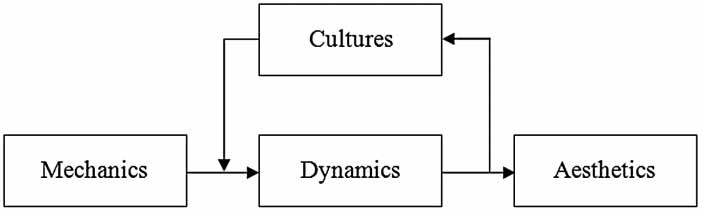
\includegraphics[width=\linewidth]{images/image01.png}
\caption{The interplay of mechanics, dynamics, aesthetics, and culture that is used to inform a game's design.}
\label{figure:mdaculture}
\end{figure}




The mechanics drive the dynamics because they constrain the actions the player may take. However, the player also has a highly influential role in the formation of the game dynamics, since games typically provide players with a choice of possible actions. Further, the skills of some players may be insufficient to sustain certain dynamics, while other players discover subversive ways to exploit the available mechanics in ways that designers may not have anticipated. These different dynamics can have a profound effect on the resulting aesthetic of the game. Again, there is variance. For example, solving a puzzle may evoke satisfaction and pride. However, if the puzzles are too repetitive, they may evoke boredom and annoyance. Players can also differ in the way they perceive an experience. Figure \ref{figure:mdaculture} illustrates an adaptation of MDA, where Scott~\cite{scott2012-monument} proposes culture as a moderating factor alongside dynamics. On the one hand, culture may shape a player's behaviour, while on the other, culture may shape a player's values and thereby influence how they interpret signs and symbols to construct meaning. Hunicke et al.~\cite{hunicke2004mda} state:

\begin{quote}


``From the designer's perspective, the mechanics give rise to dynamic system behavior, which in turn leads to particular aesthetic experiences. From the player's perspective, aesthetics set the tone, which is born out in observable dynamics and eventually, operable mechanics.''\end{quote}




It is also important to highlight a game designers' focus on aesthetics. As computer science students and educators, it may be tempting to focus primarily on the mechanics, since art, sound, and user interface design are typically not components of computer science education. However, the aesthetics are often what makes a game fun and more engaging, and considering aesthetics can be pivotal to a game's success. \subsubsection{Players}


\label{section:players}

As with teaching, the target audience of a game is of primary consideration. Players moderate the aesthetics of the games they play, as their value systems will shape their interpretations, and different dynamics may be accessed by different demographics~\cite{yee2006motivations, scott2012-monument}. Several player models have been considered and used in designing games for different target demographics. Each of the following player models with various levels of complexity have been used to identify player preferences, providing information to the designers who can then integrate those preferences within their game. Though not a comprehensive list, this provides some insight into how to consider player preferences within gameplay. When designing a game, designers can link gameplay features to specific player preferences to achieve specific goals. For example, a game designer's target demographic may be achievers, who are known to enjoy competition and the ability to achieve high scores and earn rewards. 



{\em Bartle's Taxonomy. }The Bartle's Test was developed by Andreasen and Downey, who based it on Richard Bartle's player type analysis~\cite{bartle2003designing}. This test is a questionnaire that was originally designed for players of virtual worlds to take to provide insight into their preferred play style. Four play styles are provided: Killers, Achievers, Socializers, Explorers~\cite{bartle1996hearts}. Also referred to as Hearts, Diamonds, Clubs, and Spades, Bartle attempted to classify player preferences in an effort to predict players who may enjoy dungeon crawlers. Socializers (hearts) enjoy forming relationships with other players within a game. Achievers (diamonds) enjoy meeting goals in games and being rewarded for their efforts. Killers (clubs) enjoy dominating others in gameplay using in-game means. Explorers (spades) enjoy games that provide them with an opportunity to explore and enjoy free-play. These styles are not mutually-exclusive, and in fact, players often enjoy combinations of these styles.



{\em BrainHex.} The BrainHex~\cite{brainhex} is a broader model that defines seven player archetypes based in part on neurobiological research: Seeker, Survivor, Daredevil, Mastermind, Conqueror, Socialiser, and Achiever~\cite{nacke14}. More closely aligned with genres than Bartle's Taxonomy, it can still be used as a tool within a target demographic (e.g. girls aged 10--13 in a particular middle school setting) to help in determining the types of games they may prefer, thereby creating a game to meet the preferred player styles of that demographic.



{\em Unified Model. }The Bartle's Test has been further adapted to include the Keirsey Temperaments and the Bateman DG1 Model in a Unified Model, as well as the alignment of these models with 7 others~\cite{stewart11}. This also maps to the MDA framework of game design, which defines a game based on Mechanics, Dynamics, and Aesthetics. Motivation between the different types of players as well as their preferred method of solving problems to achieve goals differs. Their overall goals (Do, Have, Know, or Become) provide a single action word summary into their play styles.



{\em Five Factor Personality Traits}{\em . }More recently, the Five Factor Personality Traits survey, a validated instrument used in psychology, has been used to predict game play preferences and in designing games. Game designers at Ubisoft employ the Five Factor Personality Inventory (also called OCEAN or the Big Five) to measure five opposing dimensions in an individual's personality, Openness (versus Closedness) to Experience, Conscientiousness versus Lack of Conscientiousness, Extraversion versus Introversion, Agreeableness versus Hostility, and Neuroticism versus Emotional Stability~\cite{vandenberghe12fivedomains}. The Inventory has been used in one study to show to that ``conscientiousness was negatively correlated with perceived use of first-person shooter games and extraversion was positively correlated with both liking and perceived ease of dancing games. Agreeableness was positively correlated with liking of dancing games''~\cite{degraft2013relating}. An alternative to OCEAN is HEXACO, which assigns personal characteristics through Humility (H), Emotionality (E), Extraversion (X), Agreeableness (A), Conscientiousness (C), and Openness to Experience (O)~\cite{lee04psychometric}.



{\em Other psychosocial models}. Though there are several ways to define player styles, other psychosocial models can be used. For example, Hofstede's cultural model has four dimensions: power distance (weak or strong), uncertainty avoidance (weak or strong), individualism (versus collectivism), and masculinity (versus feminism)~\cite{hofstede11dimensionalizing}. One could form the basis for analyzing player styles and preferences using such models. 



These models encourage examining player preferences often based on personality, in a very similar way that culturally relevant pedagogy theory is used to develop curriculum~\cite{ladson1995toward}. These models move beyond personal biological identities, with gender, race, and ethnicity, for example, not given consideration. In a classroom with learners, however, additional considerations may need to be made: environment, socioeconomic influences, instructor abilities and motivation, and more~\cite{hainey2010using}. If seen as a tool or only one form of several medium used in the classroom, games should also be contextualized by the instructors. That is, the instructor is still in control of the the learning process and interpreting the in-game learning externally provides a method of instructors integrating this knowledge---which is also referred to as pedagogical content knowledge~\cite{shulman86those}.\subsection{Effect on students}


Educational games may produce a number of learning and psychological effects. These effects may be intended or unintended. We list the most relevant effects of educational games, as well as representative measures of these effects:

\begin{itemize}
\item Cognitive development. This effect can be summarized by saying that games may present an opportunity for students to learn more deeply. For example, according to Bloom's taxonomy~\cite{anderson01taxonomy}, there are six levels of increasing cognitive development, or according to the SOLO taxonomy~\cite{biggs82evaluating}, a student may give responses to a task in five levels. Cognitive development can be measured by means of different variables, such as:
\begin{itemize}
\item Assessment performance.
\item Time necessary to accomplish a task.
\item Accuracy in performing a task.
\end{itemize}
\item Affective and motivational effects. This category clusters a number of subjective phenomena:
\begin{itemize}
\item Acceptance. Technology acceptance is a relevant issue in the area of work and training~\cite{davis89perceived}. Some students (especially adult learners) may refuse the use of games in education.
\item Emotions experienced. There is no universally accepted classification of emotions. Some authors have proposed a set of basic emotions, other being composed of the basic ones. Thus, Zinck and Newen argue that the four basic emotions are joy, anger, fear and sadness~\cite{zinck08classifying}.
\item Motivation. According to the theory of self-de\-term\-in\-a\-tion, there are four classes of motivation towards a subject matter or activity: intrinsic, extrinsic via identified regulation, extrinsic via external regulation, and amotivation.
\end{itemize}
\item Transversal skills or competences. In recent years, concern about these general skills has increased. Some examples are self-efficacy, communication or leadership skills.
\item Behavior change. Computing students may develop undesirable behaviors, such as cheating or hacking. Educational games can guide students to consider their behaviors in their academic and professional development.
\end{itemize}




Other effects can also be achieved with games but are not directly relevant to CSE: motor skills (e.g. motor coordination), perceptual and cognitive effects (e.g. attention, or visual or spatial skills), and physiological effects (e.g. heart rate).\section{Survey}


We examined over 100 unique games that have been or are currently available for use in teaching computing concepts. Each review consisted of inspecting available documentation and commentary and, when possible, playing the game. Using this information, we categorized each game with respect to numerous pedagogical and game characteristics~\cite{appendix}. These games were published over the last several decades, ranging from 1982 to 2016. Of the games reviewed, 34 are available commercially, 51 are freely available, and 15 no longer appear to be available. In this section, we provide a general summary of the games and a classification of the games in context of the ACM/IEEE Computer Science Curricula 2013~\cite{acm13computing}.\subsection{Summary of Games for CS Education}


With respect to the general computing topics addressed by the games, just over half (64) focus explicitly on some aspect of programming. Not surprisingly, within this group, topics typical of introductory programming classes are addressed by numerous games: arrays, assignment, data types, debugging, encapsulation, event handling, expressions, I/O, iteration, modularization, object orientation, parameters, recursion, selection, sequence, testing, and variables. There are also more specialized programming-related games that address artificial intelligence, algorithms, bottlenecks, ciphers, concurrency, critical thinking, fault tolerance, instruction sets, interprocessor communication, messaging, memory access, multiagent systems, problem recognition, registers, sorting, synchronization, tree traversal, and other topics. 



We found that 17 of the games focus primarily on computational thinking, in the sense defined by Wing~\cite{wing06computational}. Of the games that focus on neither programming nor computational thinking, the topics addressed include artificial intelligence, architecture, circuits, data types, security, sensors, and systems. As part of the review process, we attempted to identify specific learning outcomes addressed by each game through either literature or by playing the game. Though these details are provided in the online appendix~\cite{appendix}, they could not be summarized in a meaningful way.



We characterized the games in terms of the e-Learning Goals they claimed or that we inferred based on our experimentation. Using Clark and Mayer's cognitive task analysis~\cite{clark11elearning}, we identified ``Inform'' level goals for almost half of the games (55), ``Perform Procedure Tasks'' for more than half (73), and ``Perform Strategic Tasks'' for almost half (55).



A majority of the games reviewed specify their targeted demographics in terms of either age group or educational level. All age levels from 3 to adult and grade levels from pre-K to post-graduate are covered. Classifying the games using the five stages of experience levels, novice, advanced beginner, competent, proficient, expert, a fair number of games state that the target specific levels of prior aptitude, education, familiarity, or interest in either computing or gaming~\cite{dreyfus86mind}. 61 (59.8\%) targeted novices, 59 (57.8\%) targeted advanced beginners, 23 (22.5\%) targeted those competent in computing concepts, and 2 (2.0\%) targeted those proficient in computing concepts. We found documentation indicating that two of the games (1.9\%) were created to specifically target females. 



The games reviewed include representatives of a wide variety of genres, including action, adventure, arcade, board, dance, MMO (massively multiplayer online), puzzle, RPG (role playing game), (turn-based/real-time) strategy. Likewise, the user interface styles employed vary widely, including command line, drag-and-drop, first/third person graphical (key-based, mouse-based, controller-based), and point-and-click. Finally, there is substantial variety in the game mechanics. For example, many games are either single player or competitive multiplayer, but some are cooperative multiplayer. Also, within those games that use drag-and-drop interfaces, in some cases the objects being manipulated represent machine instructions, while in others they are game-specific actions. 



Many of the games reviewed are based on established game engines, such as Bioware Aurora, Codea, LibGDX, Moai, OpenFL, Pygame, RPGMaker, Spring engine, XP, Unity, and XNA. Others are built using identified languages and libraries such as .NET, C, C++, C\#, CSS, Flash, Git SCM, HTML, iOS, Java, Javascript, Logo, Lua, Ruby, Scratch.\subsection{Games mapped to CS 2013 Categories}


We analyzed the games in context of the ACM/IEEE Computer Science Curricula 2013 to identify which of the 18 computing knowledge areas that each game targeted~\cite{acm13computing}. For the games that we were able to classify, the majority (75.5\%) could be used in teaching Software Development Fundamentals (SDF). Nearly one-third (28.4\%) taught Algorithms and Complexity (AL) concepts. Table \ref{table:knowledgearea} shows the breakdown of the categories. Note that some games could be used to teach concepts in two or even three categories. Additionally, it is worth noting that none of the games reviewed target the following areas: IM (Information Management), NC (Networking and Communications), OS (Operating Systems), and PD (Parallel and Distributed Computing). 



\begin{table}[tb]
\begin{tabularx}{\linewidth}{|X|r|} \hline


Knowledge Areas&


Count\\ \hline


SDF (Software Development Fundamentals)&


77\\ \hline


AL (Algorithms and Complexity)&


29\\ \hline


CN (Computational Science)&


11\\ \hline


GV (Graphics and Visualization)&


10\\ \hline


AR (Architecture and Organization)&


9\\ \hline


IAS (Information Assurance and Security)&


6\\ \hline


SE (Software Engineering)&


5\\ \hline


HCI (Human-Computer Interaction)&


4\\ \hline


IS (Intelligent Systems)&


4\\ \hline


SF (Systems Fundamentals)&


3\\ \hline


DS (Discrete Structures)&


3\\ \hline


PBD (Platform-Based Development)&


2\\ \hline


SP (Social Issues and Professional Practice)&


1\\ \hline


PL (Programming Languages)&


1\\ \hline
\end{tabularx}
\caption{Number of Games classified in CS knowledge areas.}
\label{table:knowledgearea}
\end{table}




We analyzed this further and drilled down to the concept areas. The vast majority of the games target concepts in the SDF category. Within the three concept areas targeted in SDF, the concept areas of Fundamental Programming Concepts (46 or 45.1\% of all games reviewed), Algorithms and Design (25 or 24.5\% of all games reviewed), and Algorithmic Strategies (19 or 18.6\% of all games reviewed) have the most games suitable for teaching these concepts (Table \ref{table:categoryandarea}).



\begin{table*}[tb]
\begin{tabularx}{\linewidth}{|X|X|r|} \hline


Knowledge Area&


Concepts&


\#\\ \hline


AR (Architecture and Organization)&


Digital Logic and Digital Systems&


1\\ \hline
\multirow{3}{*}{AL (Algorithms and Complexity)}
&


Algorithmic Strategies&


19\\ \cline{2-3}
&


Fundamental Data Structures and Algorithms&


10\\ \cline{2-3}
&


Advanced Data Structures, Algorithms, and&


1\\ \hline
\multirow{2}{*}{AR (Architecture and Organization)}
&


Machine Level Representation of Data&


2\\ \cline{2-3}
&


Assembly Level Machine Organization&


1\\ \hline


CN (Computational Science)&


Data, Information, and Knowledge&


11\\ \hline


DS (Discrete Structures)&


Basic Logic&


3\\ \hline


GV (Graphics and Visualization)&


Fundamental Concepts&


10\\ \hline
\multirow{2}{*}{HCI (Human-Computer Interaction)}
&


Programming Interactive Systems&


3\\ \cline{2-3}
&


Foundations&


1\\ \hline
\multirow{4}{*}{IAS (Information Assurance and Security)}
&


Security Policy and Governance&


1\\ \cline{2-3}
&


Network Security&


2\\ \cline{2-3}
&


Threats and Attacks&


1\\ \cline{2-3}
&


Cryptography&


2\\ \hline
\multirow{2}{*}{IS (Intelligent Systems)}
&


Basic Search Strategies&


2\\ \cline{2-3}
&


Fundamental Issues&


1\\ \hline
\multirow{2}{*}{PBD (Platform-Based Development)}
&


Game Platforms&


1\\ \cline{2-3}
&


Web Platforms&


1\\ \hline


PL (Programming Languages)&


Object-Oriented Programming&


1\\ \hline
\multirow{3}{*}{SDF (Software Development Fundamentals)}
&


Fundamental Programming Concepts&


46\\ \cline{2-3}
&


Algorithms and Design&


25\\ \cline{2-3}
&


Fundamental Data Structures&


3\\ \hline
\multirow{4}{*}{SE (Software Engineering)}
&


Tools and Environments&


1\\ \cline{2-3}
&


Software Project Management&


2\\ \cline{2-3}
&


Software Verification and Validation&


1\\ \cline{2-3}
&


Software Reliability&


1\\ \hline


SF (Systems Fundamentals)&


Computational Paradigms&


3\\ \hline


SP (Social Issues and Professional Practice)&


Security Policies, Laws and Computer Crimes&


1\\ \hline
\end{tabularx}
\caption{Games by Category and Area.}
\label{table:categoryandarea}
\end{table*}




Based on prior evidence that games are useful for inspiring student interest, it is natural that most of the games are designed for beginners, and thus SDF and AL, which include many basic and introductory topics to computer science, would include the vast majority of the CS educational games. However, we note that there are considerable areas with few or no games that teach these concepts, leaving a wide variety of subjects that researchers could target in future games.\section{Case Studies}


Of the games that were evaluated by the group, we selected and performed a more rigorous analysis on four: The Foos, Human Resource Machine, Lightbot, and PicoBot. These games were chosen to represent well-designed games across a range of demographics, their quality, and their usefulness in appearing to meet their stated learning outcomes. We use these games as lenses into the array of games for computer science education, first describing each game using the MDA model and then comparing and contrasting the four in an effort to gauge how design elements affect the player's experience. This review serves as a backdrop for the next section in which we provide suggested best practices for designing games for use in computing education.\subsection{The Foos}


The Foos{\em , }a commercial game developed by codeSpark~\cite{codespark}, teaches basic programming concepts to students 5-10 years old. The game is available for iOS and Android. A simplified version can be played online. This game is endorsed by Code.org as an activity for the Hour of Code~\cite{codeorg}.





\begin{figure}[tb]
\centering
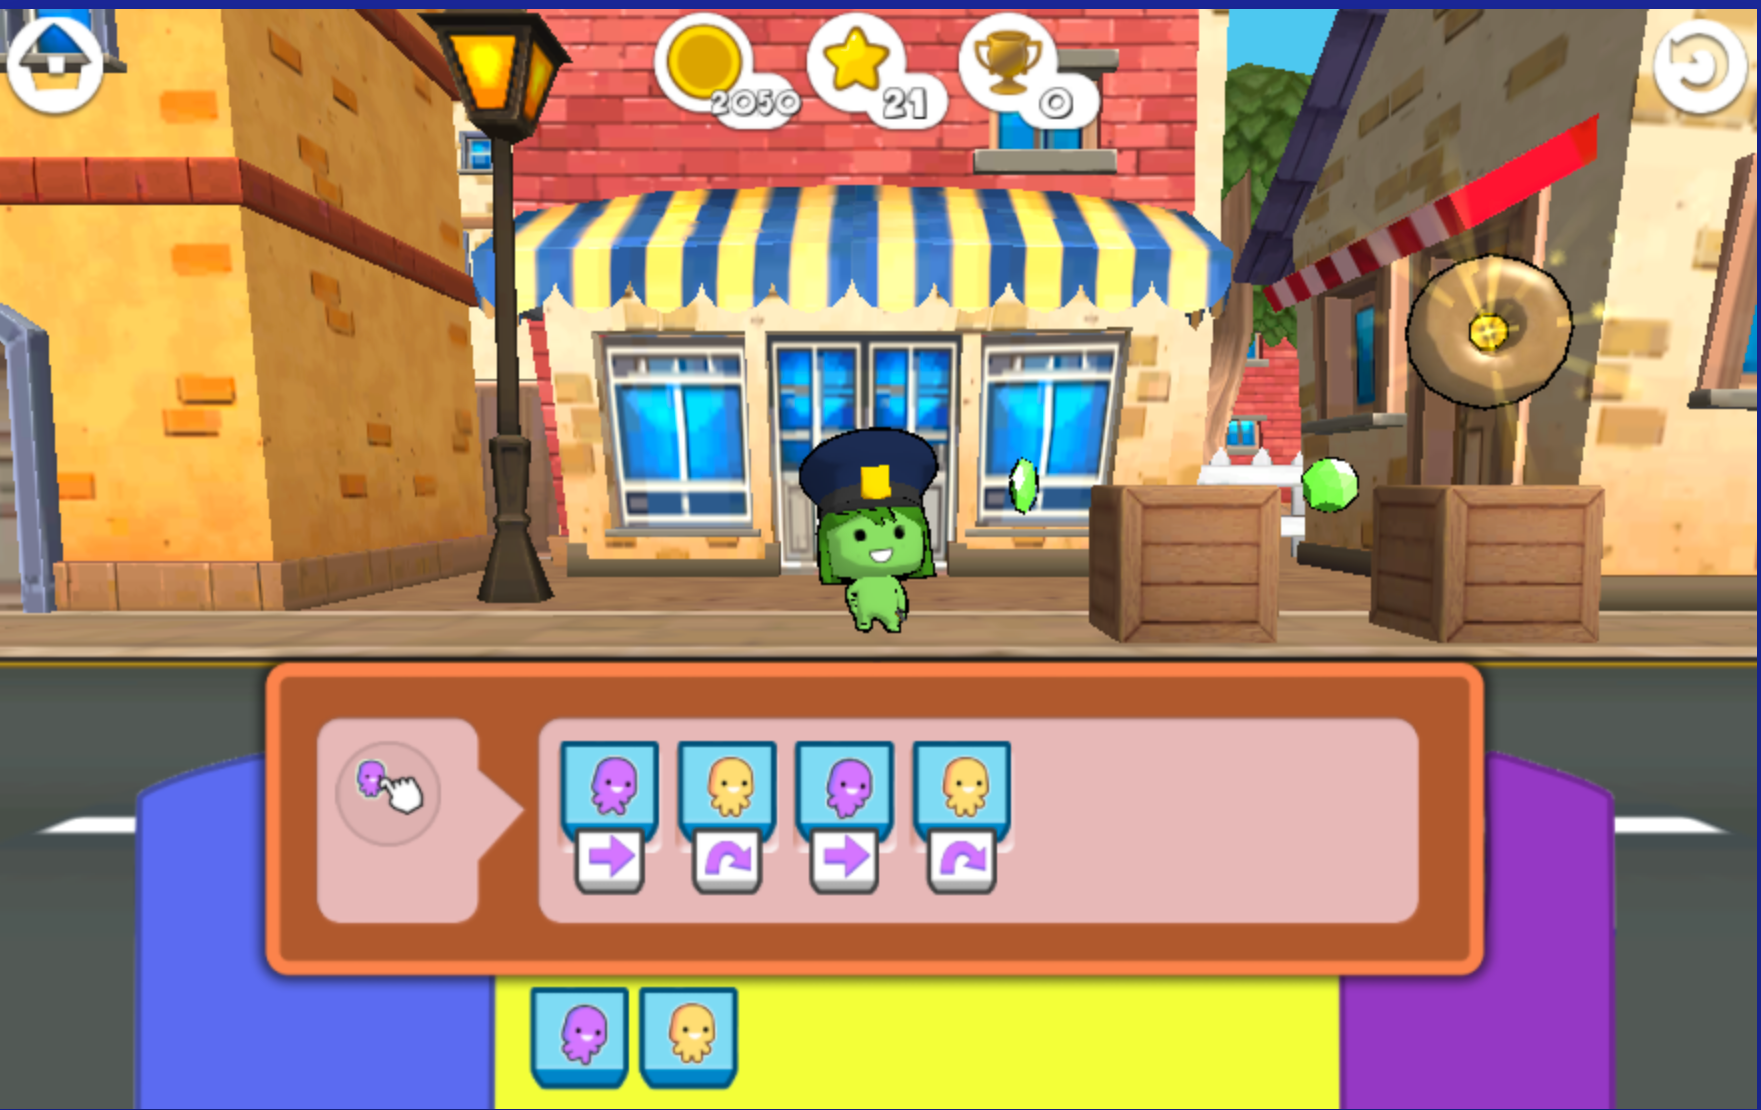
\includegraphics[width=\linewidth]{images/image06.png}
\caption{The tile-based programming editor that a player uses to guide the avatar to the donut in early level in the The Foos.}
\label{figure:fooscode}
\end{figure}


The Foos presents the player with a series of scenes featuring an avatar, some obstacles, some bonus rewards, and a final prize. The player constructs a series of moves her avatar can make in order to capture the prize. For example, in Figure \ref{figure:fooscode}, the avatar must jump on and off the wooden boxes in order to get the donut. The green collectibles are bonus rewards the player can collect along the way to the goal. For this level, the available instructions are {\em move} and {\em jump}. After constructing an appropriate sequence of steps, the player runs her program, which steps through the programmed movements with playful sound effects and music. 



If the avatar reaches the prize, the avatar dances a victory jig, while points accumulate in the heads-up display shown in Figure \ref{figure:fooshud}. If the player constructs an erroneous sequence, the avatar still follows the instructions but does not reach the final prize. The player is allowed to modify the instruction sequence without penalty until she meets the goal.





\begin{figure}[tb]
\centering
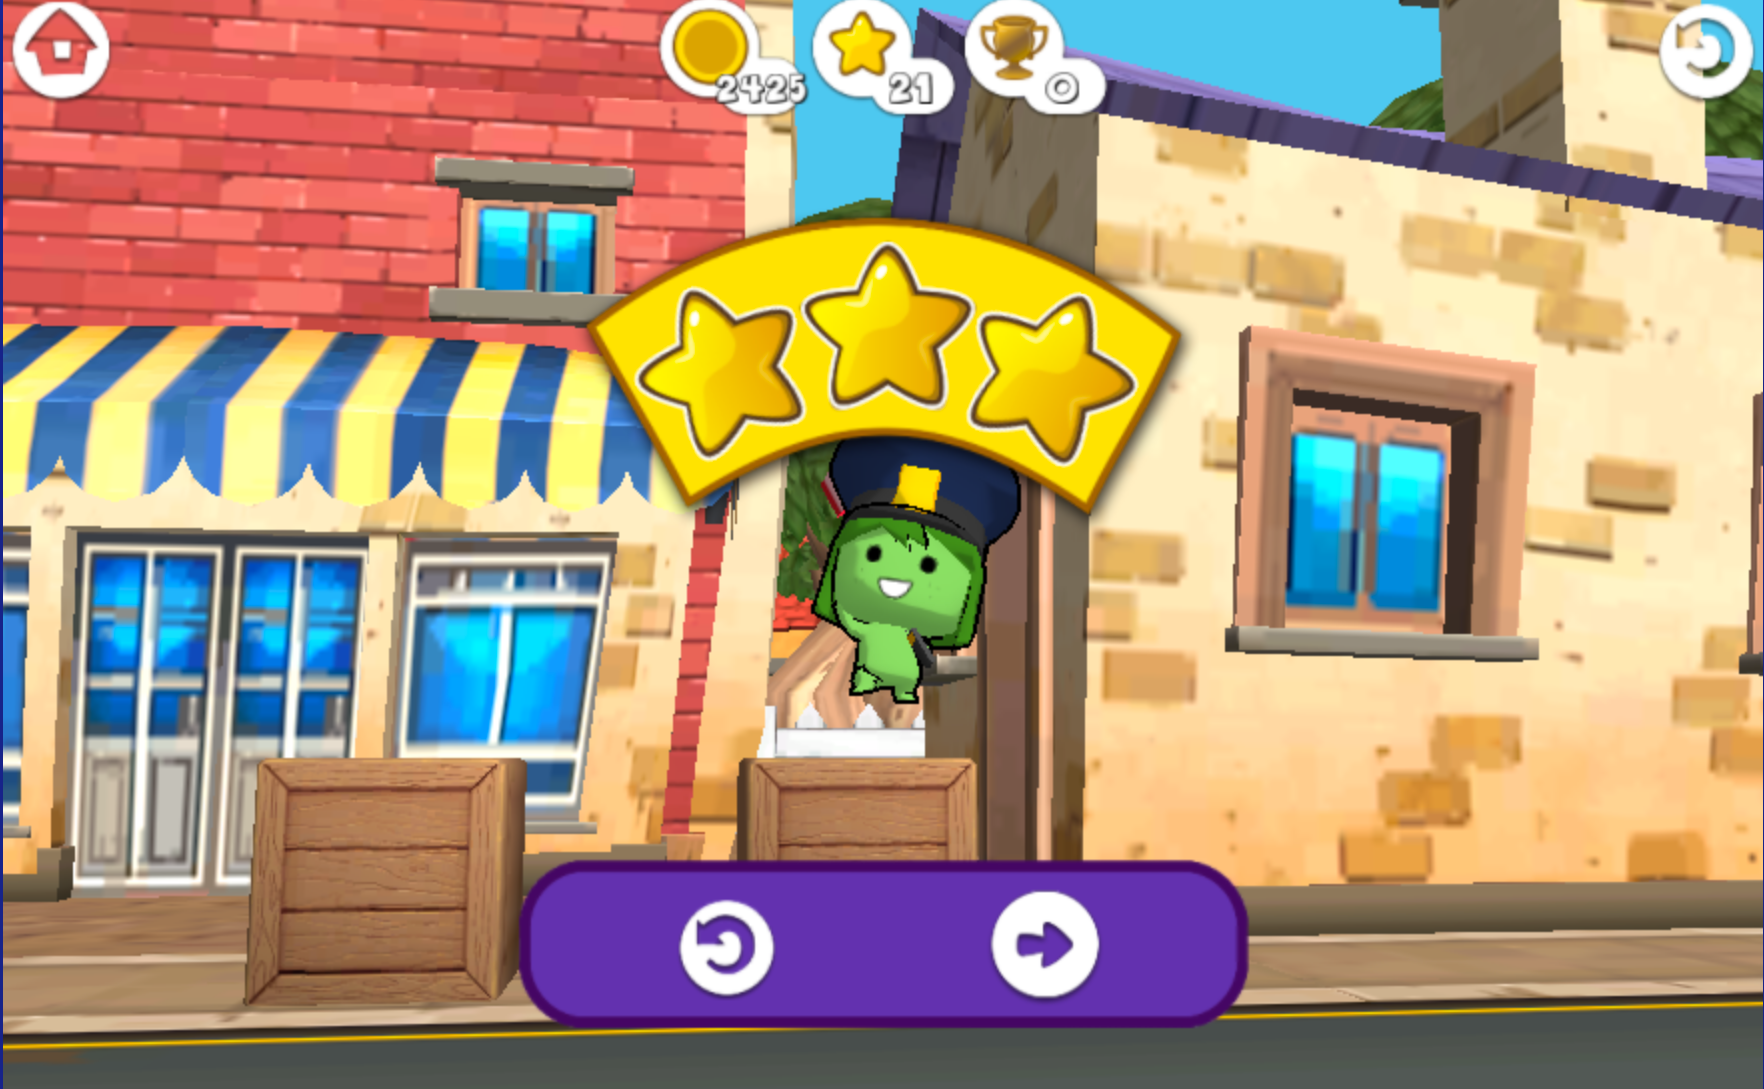
\includegraphics[width=\linewidth]{images/image00.png}
\caption{The heads-up display that reports the player's achievements in The Foos.}
\label{figure:fooshud}
\end{figure}


Since the game is aimed at young children, it does not require reading skills. It provides visual hints to help the player understand the drag and drop interface and how the available instructions work. This also makes the game easily played by students whose first language may not be English.



As levels progress different types of instructions are introduced that allow the player to solve increasingly difficult puzzles. The game incorporates 10 different scenarios, each with specific learning objectives: sequences, commands, parameters, events, loops, efficiency, endless loops, conditional statements, and debugging.



\subsection{Human Resource Machine}


Human Resource Machine is a commercial game published in 2015 by Tomorrow Corporation~\cite{tomorrowcorporation}, which is available for Windows, Mac, Linux, iOS and Android platforms. It is targeted for players age 9 and above. 



The game opens outside the drab-colored office building, whereupon the player chooses an employee avatar with large blinking eyes, dressed in a desaturated suit. Instead of choosing a name, the player chooses an impersonal employee number. 



Work begins at once for this employee, who appears in a room with two conveyor belts. One belt is marked ``In'' and the other ``Out.'' A manager sitting at a desk gives the employee her first task: move all the boxes from In to Out. While the look and feel of Human Resource Machine is very different than The Foos, the game mechanics are quite similar. The player must construct a sequence of moves the employee can follow to accomplish the objective. 



In the first level the available commands are {\tt ->inbox} and {\tt outbox->}. The former causes the employee to pick up a tile from the input conveyor belt and the latter causes the employee to place the tile she is holding on the output belt. The player drags and drops instructions to create a sequence in the program editor panel on the right. When the command sequence is executed, the employee runs between the two belts, picking up and dropping off tiles as directed. The interface is shown in Figure \ref{figure:hrmfloor}.





\begin{figure}[tb]
\centering
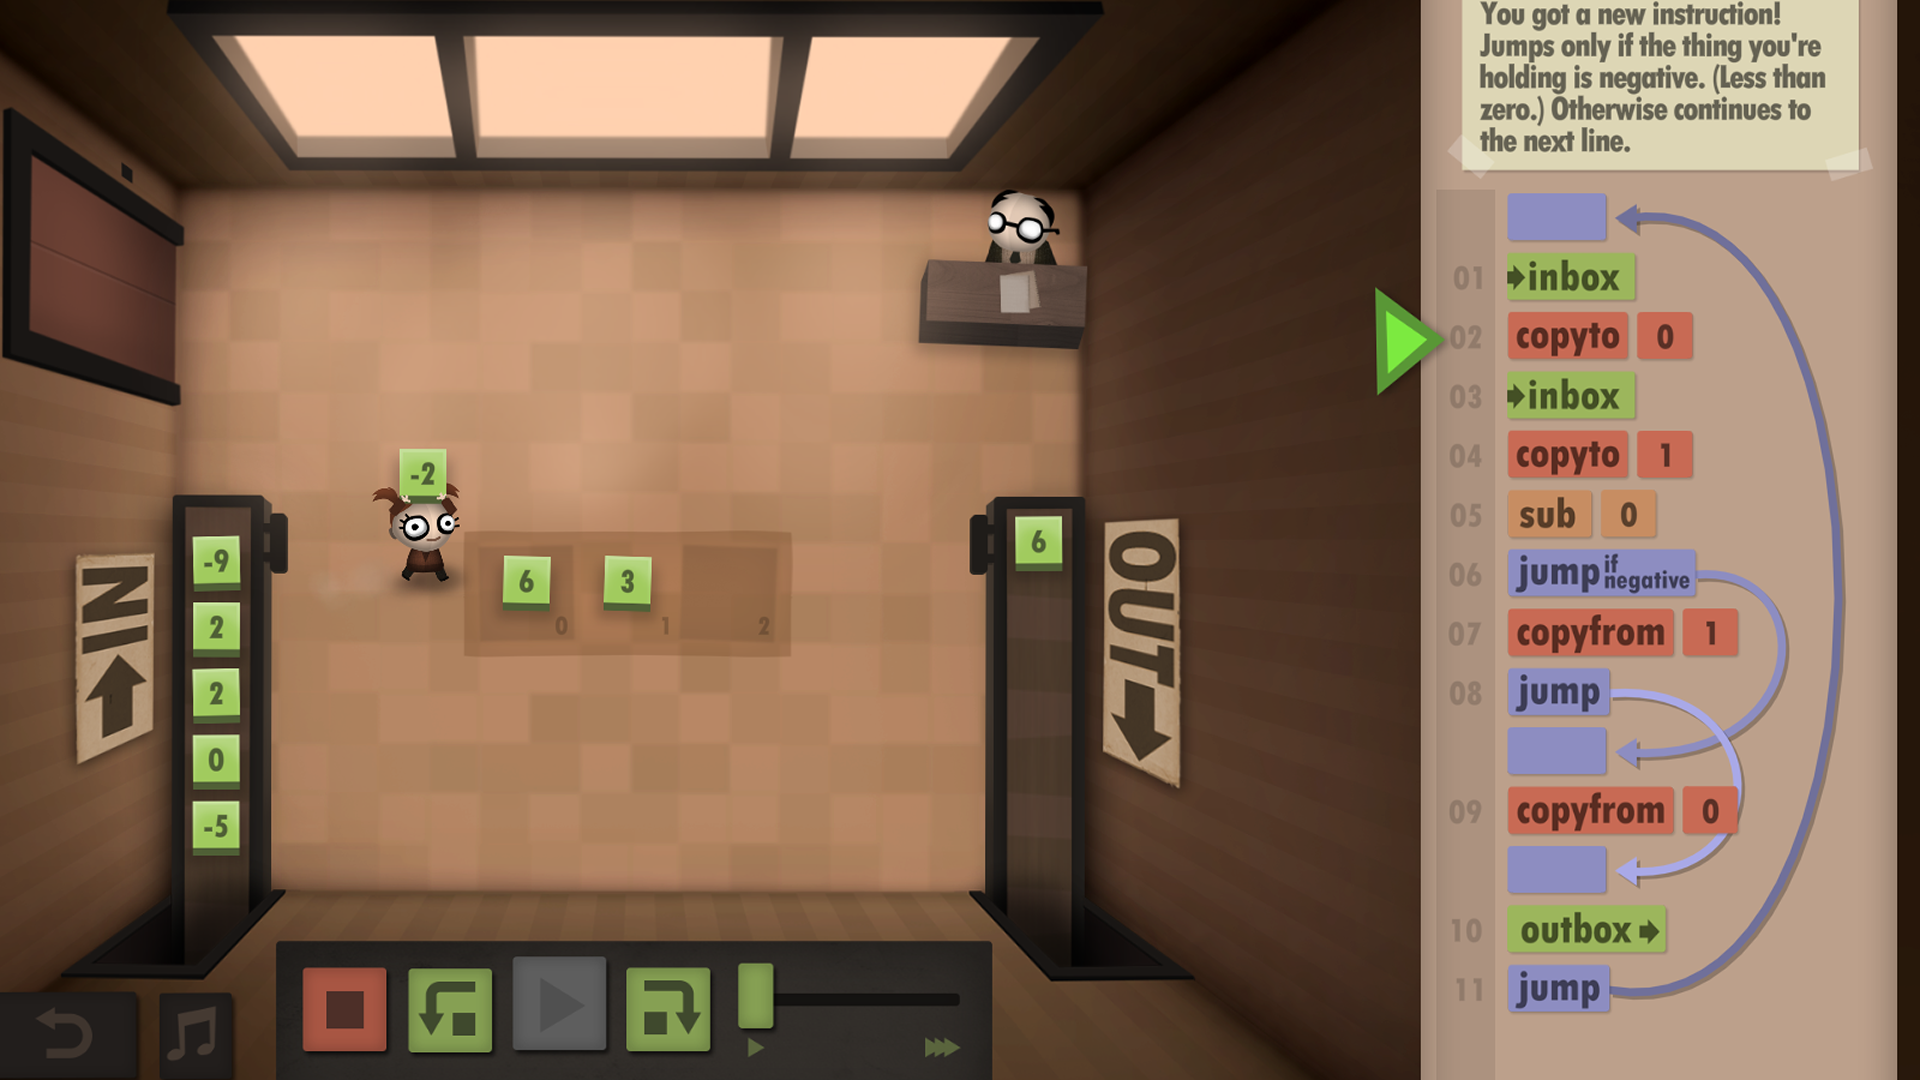
\includegraphics[width=\linewidth]{images/image03.png}
\caption{The avatar executing an assembly program that outputs the maximum of each input pair.}
\label{figure:hrmfloor}
\end{figure}


If the player fails to compose a sequence that outputs the expected tiles, the manager reprimands the employee. The player modifies the sequence without penalty until the expected and actual results match, at which point, a year passes and the employee is promoted to a more complex task. The player's progress is marked on the ``corporate ladder,'' a game screen shown in Figure \ref{figure:hrmladder} that shows a vertically-oriented map of the game's levels.





In subsequent levels, new commands are gradually introduced that allow the employee to accomplish increasingly difficult operations on the input. Additional commands include jump, conditional jump, store or retrieve tiles, add or subtract tile values, increment and decrement tile values, and so on. The final ``boss'' is a sort routine.\begin{figure}[tb]
\centering
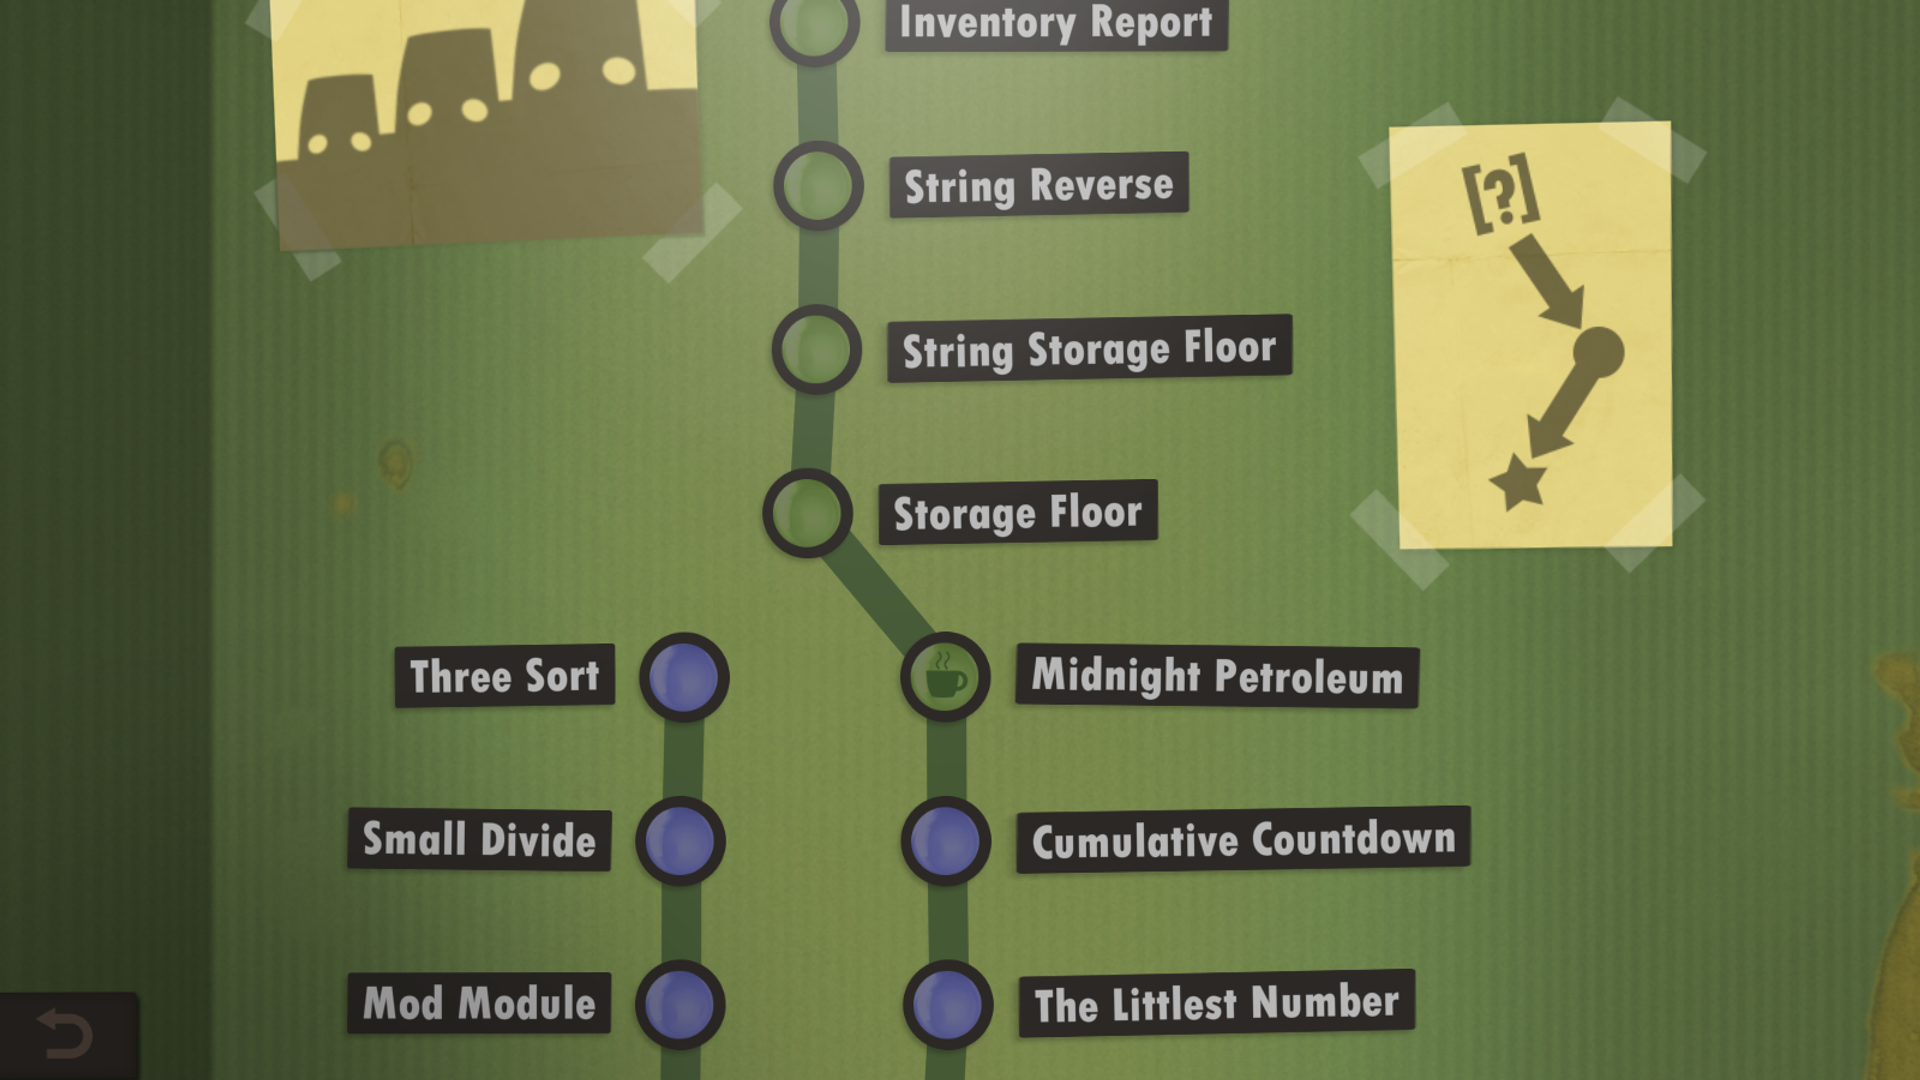
\includegraphics[width=\linewidth]{images/image08.png}
\caption{The corporate ladder that marks the player's progress in Human Resource Machine.}
\label{figure:hrmladder}
\end{figure}




When a player beats a level, a report is generated by management. The player's program is scored using two metrics: the number of instructions used in the program and the number of runtime steps required to execute it. This dual scoring reflects a tension commonly found in software development, in which one often chooses between minimizing code size and minimizing execution time. If the scores are below a certain threshold, the player's achievement is noted. The game informs the player that optimizing one metric may produce a suboptimal score for the other metric. Multiple solutions will sometimes need to be written to earn both achievements, and the player may accordingly save multiple solutions.



By the time the employee has reached the top of the corporate ladder, the player has gained fluency in an 11-instruction assembly language.



The players of Human Resource Machine are not expected to have prior programming experience, as the developers state on the game's website: ``Don't worry if you've never programmed before - programming is just puzzle solving. If you strip away all the 1's and 0's and scary squiggly brackets, programming is actually simple, logical, beautiful, and something that anyone can understand and have fun with!'' They also identify the intended audience as ``expert nerds.'' 



The developers do not discuss particular learning outcomes or assessment. However, the comments from the game's reviews on Steam provide some informal but insightful responses from players:

\begin{itemize}
\item ``Due to the fact that there is 'optimization challenges,' I do get the feeling I would return to some of the earlier puzzles to beat/match the best possible.''
\item ``Everyone will probably enjoy this game for a little while, if you like solving abstract problems and basic programming you'll enjoy it more.''
\item ``After I finished this, I realised that I'd accidentally learned how to write efficient assembly-code. Hooray!''
\item ``If you're a CS student that hasn't yet taken an assembly course, this is a great intro. The assembly language is very conventional (unlike TIS-100), so many of the skills and strategies you learn will be directly applicable to, say, MIPS or x86.''
\end{itemize}
\subsection{Lightbot}


Lightbot is a game developed by Danny Yaroslavski~\cite{openfl}, based on a game he first built in high school. It is available as an online flash game or for iOS and Android. The game comes in two versions, one targeted for players aged 4--8 and one for players age 8 and above. Lightbot is endorsed by Code.org as an Hour of Code~\cite{codeorg} exercise.



The mechanics of this game are very similar to both The Foos and Human Resource Machine. In this game the player is presented with a grid of tiles and a robot, as shown in Figure \ref{figure:lightbot}. The player constructs a sequence of moves to direct the robot to traverse the grid. Available instructions include {\em move}, {\em turn}, {\em light}, and {\em jump}. As in the previous games, the player runs the program to step through the programmed sequence. The objective of the game is to have the robot light up every dark blue tile in the grid.





\begin{figure}[tb]
\centering
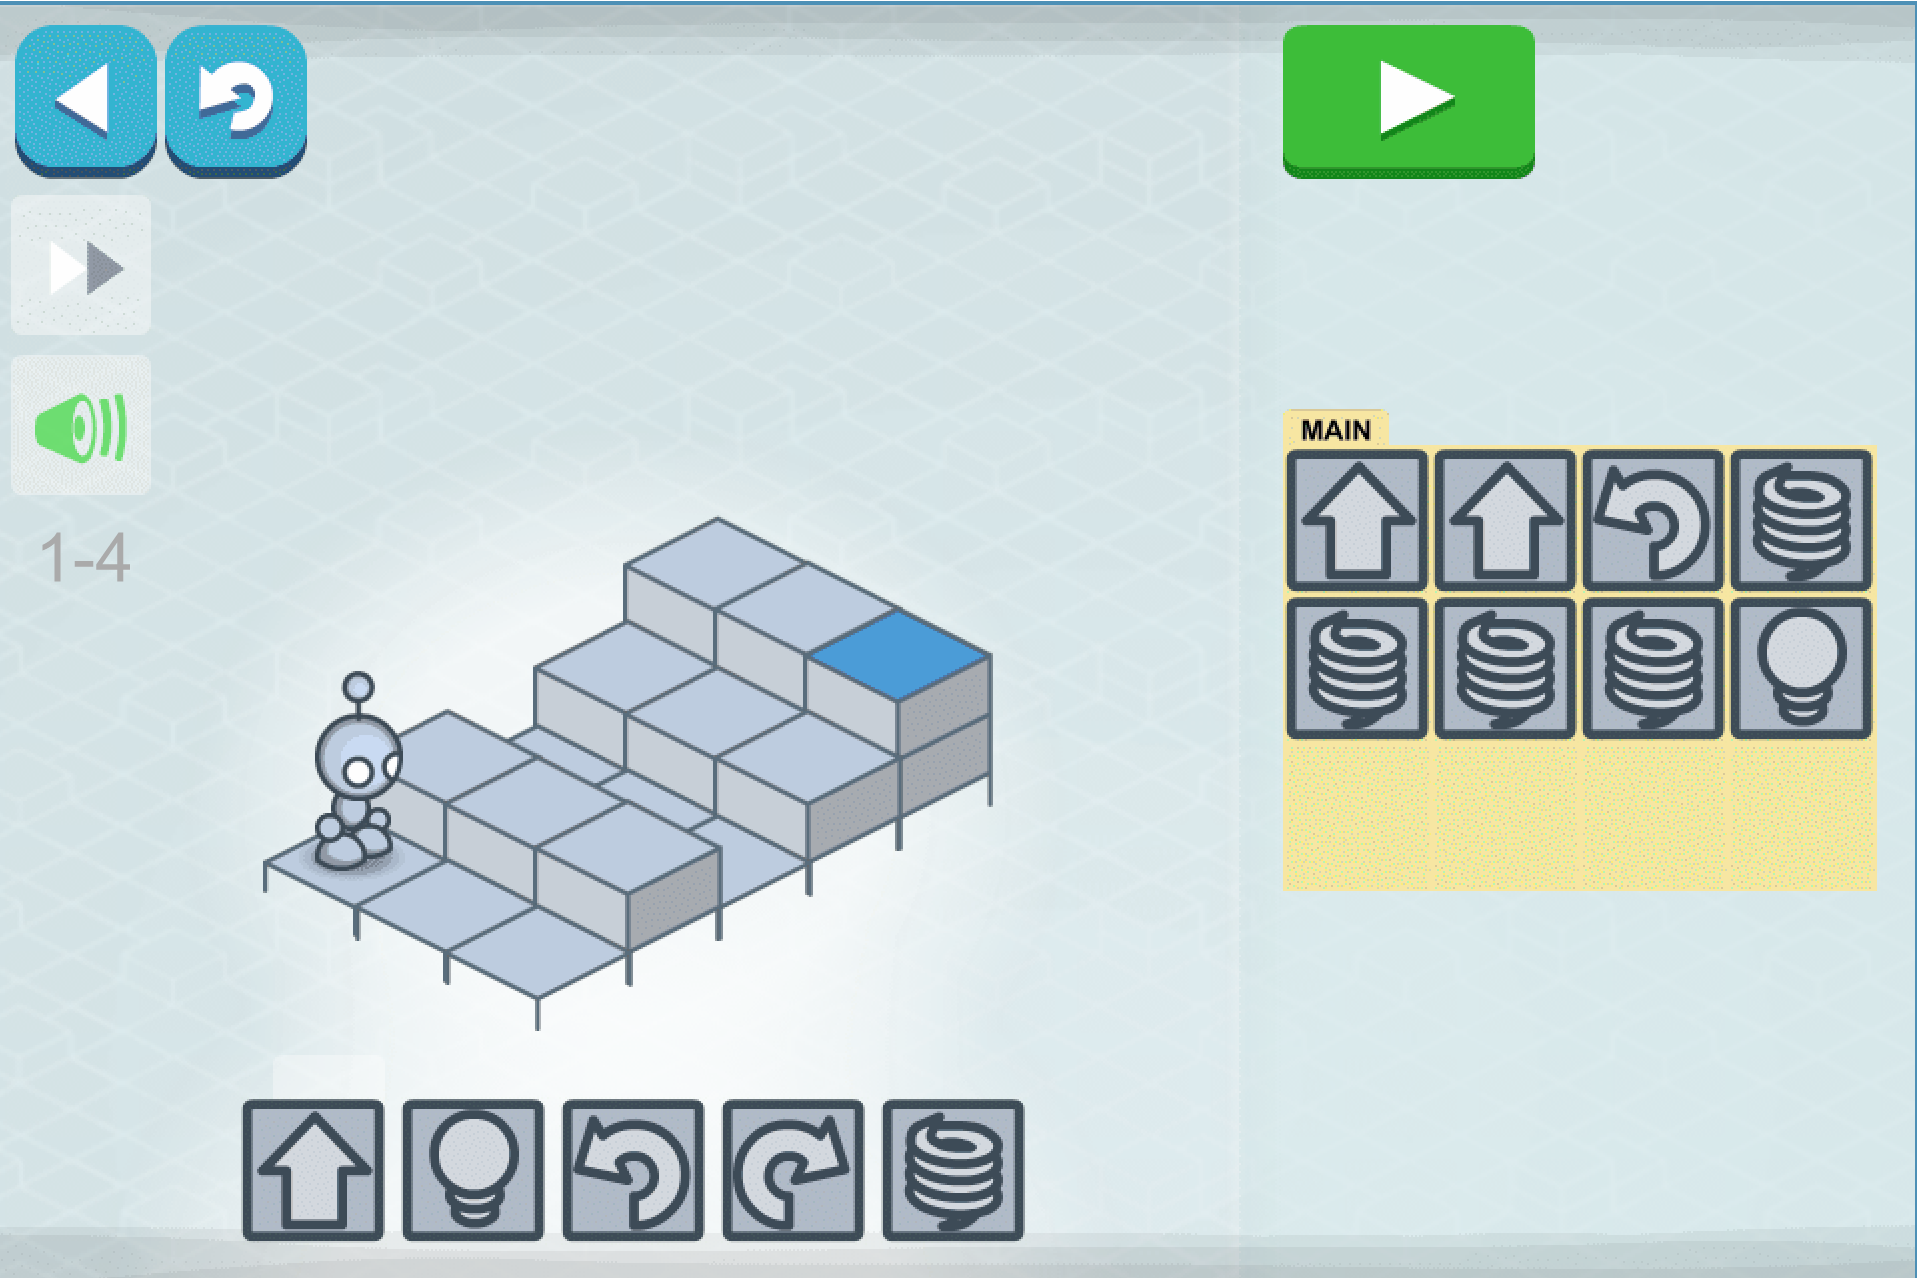
\includegraphics[width=\linewidth]{images/image04.png}
\caption{The interface of Lightbot. The player uses a tile-based program editor to navigate a robot across a world of blocks, some of which need to be illuminated.}
\label{figure:lightbot}
\end{figure}


The space provided for the tile sequences is limited, forcing the player to consider code size. As the game progresses, the size constraint adds substantial complexity to the puzzles. Similar to The Foos, if the player constructs an erroneous sequence of moves, the robot will follow its directions but will not light up all the dark blue tiles. The player can revise and rerun a sequence without penalty. Later levels incorporate subroutines and recursive calls.\subsection{Picobot}


Picobot~\cite{picobot} is a {\em Karel}-like~\cite{pattis1981karel} JavaScript game created by Zach Dodds and Wynn Vonnegut for their introductory computer science course at Harvey Mudd College. In the game, players write rules that instruct the green Picobot to navigate a two-dimensional grid world. The world consists of white, open cells that Picobot can traverse and blue wall cells that are impenetrable, as shown in Figure \ref{figure:picobot}. When Picobot visits a cell, it turns gray. The goal of the game is to have the Picobot visit all of the white cells, turning them all gray.





\begin{figure}[tb]
\centering
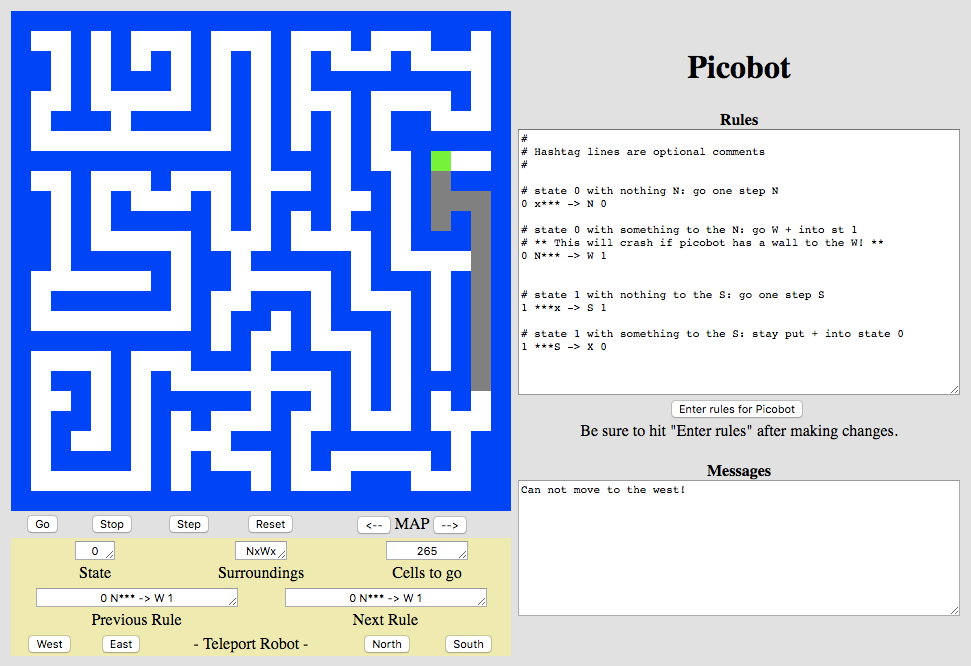
\includegraphics[width=\linewidth]{images/image02.png}
\caption{The interface for Picobot, whose 2D game world is navigated much like a Turing Machine with a 2D tape. The goal of each level is to visit all cells using only state machine rules based on neighborhood information.}
\label{figure:picobot}
\end{figure}


The game models a finite state machine. The user defines rules that dictate the Picobot's next move and new state based on the current state and which cells are in the immediate neighborhood. For example, the rule ``{\tt 0: Nxxx -> W 1}'' specifies that if Picobot is in state 0 and only its northern neighbor is barred (blue) and its other neighbors are free (white), Picobot should move west and go to state 1. An asterisk can be used as a wildcard. For example, the rule ``{\tt 1: *S** -> S 1}'' specifies that if Picobot is in state 1 and the southern neighbor is open, Picobot should move there and remain in state 1. This rule effectively moves the Picobot south as long as south is open.



Like the previous games, Picobot{\em  }introduces the player to basic programming concepts, but using a declarative programming language. It also provides visual analogy for programming problems that provides immediate, clear feedback of both success and failure. The interface also has a textual display of the current state of the program including buttons to step through the execution that is helpful for debugging. {\em Picobot} has multiple maps with various levels of difficulty that encourage players to seek and solve additional challenges. 



Picobot is not polished to the same degree as the previous games. Players enter rules using the keyboard. Its error messages can often be inscrutable to novice programmers. Picobot{\em  }does not provide hints or have a builtin tutorial. It is intended to be introduced in class by the instructor. \subsection{Compare and contrast}


The four games we reviewed are similar in many ways, but provide substantially different user experiences. These examples help illustrate the relationship between mechanics, dynamics, and aesthetics and how they work together to make a game unique. \subsubsection{Aesthetics}


From the player's perspective, a game is an aesthetic experience. Hunicke, LeBlanc, and Zubek~\cite{hunicke2004mda} suggest the following taxonomy for categorizing the user experience:

\begin{enumerate}
\setcounter{enumi}{0}
\item Sensation: Game as sense-pleasure 
\item Fantasy: Game as make-believe 
\item Narrative: Game as drama 
\item Challenge: Game as obstacle course 
\item Fellowship: Game as social framework 
\item Discovery: Game as uncharted territory 
\item Expression: Game as self-discovery 
\item Submission: Game as pastime
\end{enumerate}




This list is not meant to be exhaustive and for the purposes of educational games we can add a ninth experience:

\begin{enumerate}
\setcounter{enumi}{8}
\item Learning: Game as learning tool
\end{enumerate}




These experiences are not mutually exclusive, in fact, games typically aim to deliver on many of these objectives. 



All four of the games we reviewed provide challenge. In each case the difficulty of the challenge is targeted to a specific age group/audience. 



The Foos and Human Resource Machine both have a narrative structure. It is strongest in Human Resource Machine where the player is likely to empathize with the hapless employee trapped in the dreary corporate world. In contrast the narrative structure of The Foos is simple and fun and clearly more appropriate for a younger audience.



All games provide some sort of sensation. The Foos and Human Resource Machine use high quality graphics and sound to create a rich sensation in the player. One can hardly resist being drawn into the joyous world of The Foos with its fun characters, bright graphics, fanciful animations, and cheerful sounds. In contrast Human Resource Machine uses desaturated colors, repetitive and mechanistic sounds, and mournful characters to convey the dreariness of the corporate world (and the advantages of automation). While graphics and sound are often considered superfluous in learning games, they can greatly enhance the user's experience~\cite{juiceitorloseit}.



Based on admittedly anecdotal evidence, all of our games we reviewed are effective learning tools for their specific learning objectives and the audiences they target. The Foos and Human Resource Machine provide a richer user experience than Lightbot and Picobot. But that is somewhat essential since they are teaching children programming concepts. The fun of Lightbot and Picobot is derived largely from solving difficult puzzles, which is perfectly fine for an older and possibly captive classroom audience. Who would play if the games weren't fun? But that richness is not always easy or inexpensive to achieve. \subsubsection{Dynamics}


Game dynamics work to create the user experience. In these games, challenge is created by the difficulty of the puzzles the player must solve. The sense-pleasure of these games is tied to how effectively the game helps players navigate its challenges.



Each of the games has a progression of difficulty. The Foos, Human Resource Machine, and Lightbot introduce new mechanics across levels. Picobot has a fixed set of tools that are available from the start but the maps become more difficult to navigate over time.



Each of the games is effective in revealing state information to the player the game interface. The Foos, Human Resource Machine, and Lightbot provide a visible action associated with each command the player enters; a player can typically determine what went wrong and debug their code appropriately. Picobot's state machine simulation is more complicated but the game provides excellent debugging tools that let the player step through the state machine they have created.



The Foos has the most sophisticated in-game help systems with visual hints that help the player proceed. Human Resource Machine and Lightbot have non-player characters that provide directions. Picobot does not have in-game instruction. While some players may be able to figure out the gameplay on their own, many will require an instructor's guidance.



All of the games tolerate some variation in the successful solutions. The Foos is particularly forgiving about missteps; an incorrect sequence played twice (without reset) will often have enough correct moves to achieve success. Because Human Resource Machine has two scoring metrics, it actually encourages players to consider alternative solutions; this contributes to aesthetic goals of Discover and Expression. Similarly, Lightbot grids often have numerous solutions though the constraint on sequence length can limit possibilities. Picobot provides the least constraints on the solution space; for some players this may be liberating but it also allows for complicated solutions that are difficult to debug. But once again, Picobot is intended for classroom use where an instructor can help get students past difficult hurdles.



Each of the games encourage computational thinking by initially focusing on simple problems the player must solve through a series of simple steps. Later levels provide more difficult problems and, in the case of the first three games, provide advanced techniques like recursion to help solve them. \subsubsection{Mechanics}


Mechanics are the rules of the game and the actions and controls available to the player. The first three games have very similar mechanics; the player drags and drops instructions to creates a sequence their avatar follows to achieve some goal. This provides a good introduction to imperative programming.



Picobot is different than the other three games in that its rules are defined using a declarative programming language, which may not be appropriate for classrooms that focus on imperative programming. But this difference can also be a strength, particularly an introductory computer science course that aims to expose students to multiple programming language paradigms.



Human Resource Machine has the most sophisticated scoring system providing two separate metrics by which a solution can be evaluated: code size and execution time. Lightbot only focuses on the first of these metrics but does so with a very hard constraint; limiting the space to describe a solution effectively limits the player to efficient solutions. The Foos scoring system is the most forgiving; even wrong solutions can garner points. This is appropriate given its young target audience. \subsubsection{Summary}


We consider each of these games to be fun learning tools for their intended audiences, and as such each has the potential to be effective. Games developed by professional designers/developers with access to considerable resources are going to have greater polish. But simple games that are designed for specific use in a classroom can be highly effective in their own right and, therefore, should be considered as another tool for enhancing learning.\section{Suggested practices for designing games for use in CS education}


Based on our review of games, our experience as computer science educators, our understanding of educational research, and our experience designing and developing games, we provide considerations for designing games for use in computer science education. We discuss useful and relevant aspects of educational frameworks to consider when designing, basic game production practices to aid a researcher new to game design, and methods for enhancing the player (student) experience. This is followed by techniques for integrating games into curriculum. Though not an exhaustive list, we propose that these are useful starting points for creating games for use in CS education. \subsection{Infusing Educational Frameworks}


Hainey's dissertation~\cite{hainey2010using} considers a set of seven factors that influence learning in the context of games. These are shown in Figure \ref{figure:haineyframework}. Each of these categories of influencing variables are further defined by Hainey to provide a reference for evaluation methods, and each is important for instructors to consider the impact of games as a learning tool. Like books, videos, and other teaching tools, their impact is often heavily influenced by many other factors. 





\begin{figure}[tb]
\centering
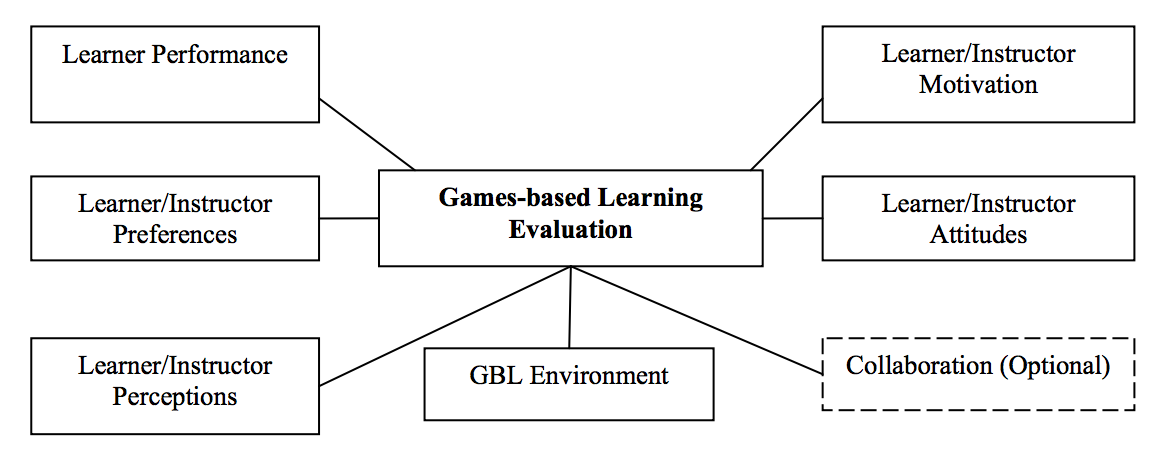
\includegraphics[width=\linewidth]{images/image07.png}
\caption{Hainey's evaluation framework for games-based learning evaluation.}
\label{figure:haineyframework}
\end{figure}
 

 

However, although striving to evaluate a newer media is a desirable goal, holding a formal evaluation of games as a litmus test for whether or not they should be used for learning contradicts what instructors do in classroom preparation each day. Shulman~\cite{shulman86those} refers to this as the ``wisdom of practice,'' or the practice of instructors to choose assignments, activities, discussion questions, lecture topics and more based on their knowledge and wisdom of the content and how their particular set of students learn. In considering wisdom of practice, games can be carefully selected by instructors to incorporate them into their curriculum in meaningful and influential ways.



Many games for learning may be used as stand-alone games for independent learning by the learners; however, providing context for the learner's in-game experiences is certainly part of the game-based learning environment~\cite{oneil05classification}. The manner in which the instructor integrates the learning experience from games into the classroom is very important to its effectiveness. 



Based on this, integrating the learning into the classroom is an important aspect of the curriculum design process, and instructors can liken themselves to the Dungeon Master (DM) in Dungeon and Dragons. The DM sets up the context for the dungeon or game. They provide assistance during the game to clarify any questions and can debrief after the game.\subsection{Important Caveats}


Though this set of guidelines is not comprehensive, it has the potential of being overwhelming for someone who has not yet created games for learning. We recommend researchers new to this field find one or two areas on which to focus, then expand those areas as more work is considered.



As previously mentioned, though our initial goal was to provide a guide for assessing games for efficacy, scope and time prevented us from engaging in that activity. This should by no means be taken to imply that this goal is not as worthy. We recognize its importance and intend to pursue that activity in whole or in part during the 2017 ITiCSE Working Group. 



We note here that beyond knowledge and skills, attitudes and dispositions are valid reasons for providing games as a learning tool in CS. Motivation, engagement, happiness, satisfaction, and perceptions of the field among students across a wide range of demographics are important aspects of games for CS education. As educators, the ``wisdom of practice'' may not be enough for this new medium, and we may be interested in various levels of proof that games are effective. A wide range of tools for understanding effectiveness can and should be used. For example, test scores, students surveys, quantitative or qualitative research methods, and/or rigorous evidence (replicated, longitudinal) are all forms of data that can be used to determine whether a game may be effective for a particular group of students. 



The next two sections on game development processes and game design for games for use in CS education are presented in the context of games for CS education where possible. These two sections are also enhanced by Section \ref{section:integrating}, which discusses best practices integrating games into the CS curriculum or a CS classroom. \subsection{Basic Game Development Processes}


Game design is the process of designing the game. Game production is the process of taking the design and implementing it. There are many books and articles on game production, and in this section we highlight a few important aspects of development that a researcher newer to creating game for CS education might find useful. 



{\em Agile processes. }Agile processes~\cite{agile} are often used in managing a game project. A project is broken into tasks or sprints. In a classroom setting, the first sprint, for example, may last two weeks and during that time students may be responsible for creating a game proposal. One of the values of agile development is the reflection at the end of each sprint of what is going well with the project, what needs to be improved, and what might be standing in a team member's way. 



{\em Moodboards, Storyboards, Ripomatics.} Moodboards provide a visual representation of the art style, typography, and early visual design and themes of the game to convey its look and feel. An example is shown in Figure \ref{figure:koalamoodboard}. Storyboards provide a visual representation of gameplay and narrative. An example is shown in Figure \ref{figure:koalastoryboard}. Ripomatics are scenes that are ``ripped from'' existing media such as film, TV, or games to provide a concept of the look and feel of the proposed game. All of these can be used to create a consistent look and feel across the game and are particularly useful when multiple people are working on the game. 







 \begin{figure}[tb]
\centering

\includegraphics[width=\linewidth]{images/image05.png}
\caption{Sample moodboard for the game Wake Up, Koala!, a game developed by undergraduate students to raise awareness about Sj\"{o}gren's Syndrome.}
\label{figure:koalamoodboard}
\end{figure}






\begin{figure}[tb]
\centering
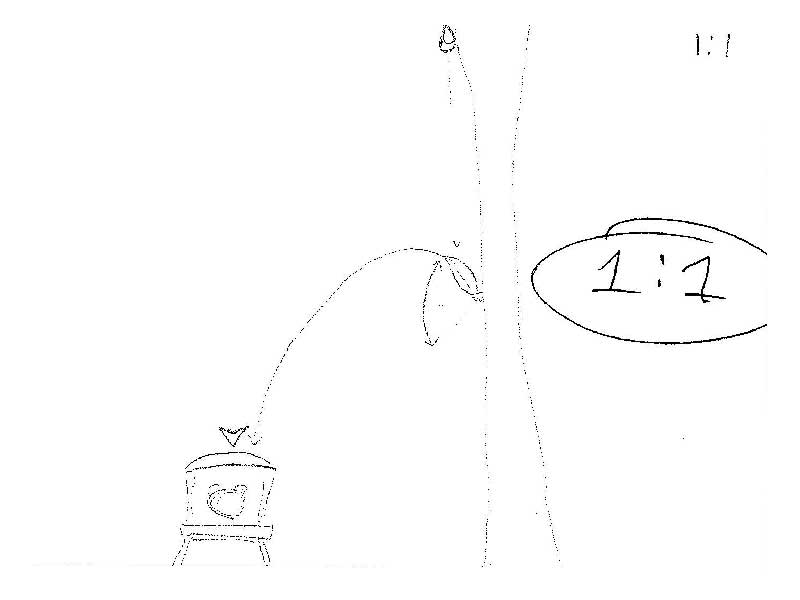
\includegraphics[width=\linewidth]{images/image09.jpg}
\caption{Sample storyboard for the game Wake Up, Koala!}
\label{figure:koalastoryboard}
\end{figure}


{\em Paper prototyping and testing.} Paper prototyping is the process of presenting a game idea through storyboards or mockups of a game's scenes (or a combination) to present your game in a paper format to potential players. This form of test has been proven to be very effective to gauge how fun is one's game, to determine whether the flow of the game is effective, and to determine if players are learning. This process enables the developers to get feedback very early in the design process, before actual production of the game begins. It is much easier to correct major issues with flow and game mechanics before starting to program rather than after time and effort has been spent on programming the early prototype of the game.



{\em Quality Assurance and User Testing.} Testing is a necessary and important process and is critical for enhancing the user experience. No one likes to have flow broken when learning due to problems with their learning aides! We have used two types of testing, one with users to gain critical feedback on concept builds, early prototypes, alpha, and beta builds. In this type of test, users are solicited for feedback on how to improve any part of the system. The other, quality assurance, is the development team's responsibility. This type of test includes the painstaking process of testing each element within the game (buttons, scene transitions, scoring, general functionality, and more) as well as art, animation, and sound. \subsection{Designing for the User Experience}


Within this section we provide a set of design principles for game development. Though not meant to be comprehensive, we carefully selected elements that are important to consider when designing a game for use in CS education. The intent is to provide a best practice cheat sheet for creating games for CS education to those newer to game design and development. This toolset considers best practices in each area and is designed to suggest methods for improving the impactfulness of the games.\subsubsection{Define the Learning Outcomes}


Games have been shown to improve learning in some computer science education domains, such as computer memory~\cite{papastergiou2009digital}. Embedding sound instructional design into games for learning is needed if we want the games to be effective. O'Neill, Wainess, and Baker~\cite{oneil05classification} note that many games for learning have historically missed the mark on this. They make the case that CRESST and Kirkpatrick's models for learning can be evaluated and applied within a game's design. 



The Understanding by Design model~\cite{wiggins05understanding} is also relevant to game design for education. The three major stages of this backward design model is to 1) identify the desired results, 2) determine the acceptable evidence, and 3) plan the learning experiences and instruction. These stages can be tailored for the development of games for computing education as follows:

\begin{itemize}
\item Stage 1:
\begin{itemize}
\item Establishing learning goals for the player 
\item Defining the set of essential questions for achieving these goals
\item Identify the understandings that are desired
\item Specifying what key knowledge and skills students will acquire as a result of playing the game
\end{itemize}
\item Stage 2: 
\begin{itemize}
\item Identify the tasks that will be performed in the game to provide the evidence needed to ascertain the player's understanding of the learning material
\item Identify any other evidence that should be collected to determine if the desired results in Stage 1 have been met. Include time playing, time spent in each level, incorrect and correct moves, etc. 
\item Provide a manner for the players to reflect on their learning experiences
\end{itemize}
\item Stage 3:
\begin{itemize}
\item Once Stages 1 and 2 have been drafted, design the sequence of experiences that the players will need to engage with in the game, develop by playing the game, and demonstrate within the game those desired understandings identified in Stage 1. 
\end{itemize}
\end{itemize}




Though there are many aspects in instructional design to consider, for both development and evaluation purposes, learning outcomes are at the top of the list. Defining the goals and learning outcomes for a game will not only provide clear direction when designing, but also provide a set of metrics for which to evaluate the game for effectiveness. \subsubsection{Research target users}


Referring back to Section \ref{section:players}, knowing the player preferences of your target learners is important when designing games. As noted by O'Neil et al.~\cite{oneil05classification}, games for learning can be effective for developing learning strategies, but ``players apply those strategies differentially, with some players more effective than others. These differences come not only from our knowledge, skills and abilities, they are socially motivated as well.'' Learner (and instructor) preferences are important variables to consider~\cite{hainey2010using}.



There has also been much discussion within the game industry that game designers have historically chosen to create games that appeal to them. Anthropy~\cite{sheffield12token}, a game designer, noted that game designers are primarily white and male, and this has influenced the types of games that they have created and has, in turn, influenced the types of players that are attracted to such games. It is important to consider the preferences of the learners one aims to target, especially in light of the continued lack of diversity within computing~\cite{national13women}. The game industry has begun to mature beyond stereotypes like ``girls like pink and boys like blue,'' recognizing that the player, regardless of their sex, may prefer an avatar that is blue or pink or another color altogether. 



The tools mentioned in Section \ref{section:background}, such as BrainHex or a Big 5 Personality Survey, can provide a starting point for the type of game that might be most engaging for a set of learners---particularly for high school and adult learners. Considering age and ability in your design choices can also make your game more effective. From a pedagogical point of view, by so doing, researchers can engage in developing a form of culturally relevant pedagogy that will be more inclined to motivate and engage learners~\cite{ladson1995toward}.



There is also value in bringing a representative group of targeted users into your design process. Whether they become part of the design process by making choices about the theme or genre, or whether they are asked for their input at various stages of the game's development, the process will help ensure that the game is engaging for the learners that they represent. \subsubsection{Engagement}


In both video games and assignments the notion of overcoming a challenge is one of the primary motivators for engagement~\cite{ryan06motivational}. The presentation of challenge must be carefully balanced to be effective. This concept is called flow in video games and scaffolding in educational delivery~\cite{cs90flow}. If the material is too hard, student-players will give up, and if it is too easy, the student-player becomes bored and will lose engagement. In both cases, as the skills of the student-player increase the difficulty of the class/game must also increase.



While there are always exceptions, assignments and video games have separate avenues for generating additional engagement for the student-player. In crafting assignments the inclusion of personal meaningfulness can provide dramatic increases in engagement. Hulleman et al.~\cite{hulleman10enhancing} asked students to write essays about how their learning of math or psychology was relevant to a student's life. Interestingly, being told by an instructor that something was good for them only helped the high ability students. When students wrote their own reasons, they were more engaged with the material. A similar technique calls on instructors to utilize socially relevant causes in order to increase student engagement and learning~\cite{buckley08socially}. Seeing direct applications of their discipline of study generates excitement in the students.



In video games, the designer can use a multitude of tools in order to increase engagement. However, not all are equally powerful. In a survey of gamers the four most reported game aesthetics (after Challenge) that increased engagement are, in order, Narrative, Fellowship, Sensory, and Discovery~\cite{schoenau-fog11player}:

\begin{enumerate}
\setcounter{enumi}{0}
\item Narrative was reported as the most common reason that players would continue playing a game. The story becomes part of the reward structure. In order to uncover the entire story, a players must typically finish a significant part of the game content. Narrative can be delivered in the form of traditional dialog elements, such as characters talking or a background story. However, the best stories are formed through the combined use of dialog, art, sound, level design, and mechanics.
\item Fellowship with other players fulfills a psychological need in people to connect with others. The desire to meet up with friends or adversaries within the game can keep players returning long after they have completed the game content.
\item Sensory aesthetic has traditionally been the use of visual and audial components to create an immersive experience. However, new technologies such as Kinect and Wii controllers have introduced the use motion as a sense pleasure. New advances in augmented realities, such as Pokemon Go, will further expand the means by which we can offer sensory aesthetics.
\item Discovery appeals to curious players who wish to discover all that their world has to offer. This can be simple exploration of the environment, but also experimentation with mechanics or unlocking all of the secrets within the game. Games which provide player agency in accomplishing goals are most likely to fuel the Discovery aesthetic. 
\end{enumerate}


\subsubsection{Positive/Negative Reinforcement}


Games are designed to shape their players. This shaping occurs at many levels, ranging from the simple cues that teach a player how to navigate a game world to the promotion of beliefs and skills that the player will carry outside the game. How exactly the player is shaped is an important ethical concern of game design.



Skinner introduced the idea of {\em operant conditioning}~\cite{skinner1963operant}, which he defined as the encouragement of behaviors through positive and negative reinforcement and their discouragement through punishment. These consequences increase or decrease the probability of the associated behavior in the subject to whom they are applied. Within a game, consequences are often delivered through game mechanics that hold significant value to the player, like scores, wealth, visual and auditory feedback, character health, and leveling systems. The feedback delivered through these tools selects out certain player behaviors while diminishing others. 



Games do much of their shaping through positive reinforcement, by rewarding a player for performing a desired task. The schedule and structure of these rewards is a key component of player engagement. In early gameplay, rewards may need to be delivered more or less continuously to draw in a player~\cite{loftus1983mind}. However, rewards dispensed continuously and without merit quickly lose their value.



To avoid this, designers soon alter the reward schedules to deliver only {\em partial reinforcement}, in which rewards are dispensed intermittently. The reward schedule may be a {\em ratio schedule}, in which the player is rewarded only after completing a certain number of actions. Alternatively, the reward schedule may be an {\em interval schedule}, in which the player is rewarded only after a certain amount of time has passed. Further, the schedule may be {\em fixed} or {\em variable, }indicating that the gap between rewards is either known or effectively random, respectively. Each combination of these two qualities leads to different profiles of gameplay. In general, a variable ratio schedule tends to keep the player most consistently engaged~\cite{hopson01behavioral}, but fixed schedules can produce bursts of activity just before the anticipated reward.



Reinforcement may be spoiled in a number of ways. Rewards not delivered in a timely manner can lead to player frustration and the {\em extinction} of the desired behavior. Rewards not valuable to the player do not have the desired effect on behavior. For this reason, games offer a variety of different reward types. A player may be content receiving a reward of small magnitude. But if one of larger magnitude is introduced, any subsequent smaller rewards are likely to be treated with disdain.



Nearly all games use some form of operant conditioning to keep the player playing. Frattesi et al.~\cite{frattesi2011replayability} identify several means of promoting replay value within a game: its difficulty should balance challenge and frustration, a player's completion status should be clearly communicated, it should draw on social aspects to facilitate community, its gameplay should have elements of randomness to produce feelings of unexpectedness and novelty, and it should provide a unique experience that cannot be found elsewhere. Educators designing games have different goals than commercial game designers, and replayability should be considered only in the context of sustaining learning. If a student has mastered a game's learning outcomes, then replayability is undesirable and the student should move on to new challenges. Game designer Raph Koster says, ``In the end, that is both the glory of learning and its fundamental problem: once you learn something, it's over. You don't get to learn it again''~\cite{koster2013theory}.\subsubsection{Reward Systems}


Reward systems can shape players towards desirable behaviors like longer game play, more effective use of time, or breadth of coverage. Points, level, badges, or virtual goods feed the player's need for status and accomplishment. Even though these artifacts do not exist in real life, digital artifacts symbolize the player's status among other players and increase their feelings of self worth. Completion bars and checklists allow users to see goals and plan out how to complete them. Leaderboards allow a person to compete with others in a competitive setting. Analytics like heat maps and histograms allow a player to monitor their performance and provide course correction for personal goals.



Many reward systems are orthogonal to core gameplay mechanics. Therefore they can be added and altered without significantly changing the original game. Because of their disconnectedness from the actual game but their profound influence on player behavior, reward systems are the core of gamification, which is the addition of game-like elements to non-games to increase engagement~\cite{muntean11raising}.



There are three caveats in utilizing reward systems to change player behavior. First, reward systems are a force multiplier and not a substitute for the interesting underlying activity. Rewards will not cause players to enjoy the underlying activity if they did not do so in the absence of rewards. However, reward systems will increase how players self-report their overall experience playing the game.



Second, not all reward systems are meaningful for all players. Hakulinen~\cite{hakulinen2015gameful} found that students responded to different rewards based on underlying goals. For instance, students with a fear of being seen as incompetent favored heatmaps, which warned how much danger they were in, compared to badges, which indicated that they had succeeded in a particular topic.



Third, be mindful that reward systems are subtle ways to affect and shape player behavior. Sometimes the behavior that you shape is undesirable. O'Rourke et al.~\cite{o2016brain} utilized reward systems in the game Refraction to reward players that used mindful approaches to problem solving. When students in the treatment group displayed mindful approaches in the game, they were awarded ``Brain Points.'' O'Rourke found that students in the treatment group did play longer. However, the control group displayed more growth mindset behaviors during game play. Reward structures can be difficult to fine tune for alternative behaviors.\subsubsection{Formative and Summative Assessment}


According to the Theory of Multimedia Learning, ``people learn more deeply from words and pictures than from words alone''~\cite{mayer2014cognitive}. This is a concept accepted by many in the computer science education community because visualizations can be used to not only engage learners but more powerfully they can make feedback of an abstract problem more concrete. Consider a middle school introduction to computer science where students write programs to create animations using Alice~\cite{dann2000making}. When a program does not produce the desired animation, the learner is given immediate and obvious feedback. Or consider a college-level computer science course for non-majors using Guzdial's media computation~\cite{guzdial2003media}, where students write programs to manipulate images. Specifying the behavior of an assigned program in such an environment may be as simple as giving before and after images.



Work by a previous ITiCSE working group~\cite{naps03exploring} concluded that visualizations alone are not a sufficient learning tool. Visualizations must be used to engage students in active learning. This conclusion is corroborated by later work showing that visualizations alone do not demonstrably show learning benefits~\cite{rieber2008games}, but a visual metaphor in conjunction with a gaming context does.

We as educators know that formative assessment, with frequent, quick, clear feedback of student work, can have a significant effect on student learning~\cite{black1998assessment}. Games are an opportunity to provide students with faster, more frequent, and clearer feedback. Formative assessment can also be used by instructors to customize the classroom experience to better utilize class time and to maximize learning opportunities. This is seen in pedagogical techniques like Just-in-Time Teaching (JiTT)~\cite{bailey2005just}, where out of class readings and quizzes are used to help make modifications to class immediately prior to class. Instructors use of formative assessment is also seen in peer instruction~\cite{simon2010experience}, where student responses to in-class clicker questions are used by the instructor to guide classroom discussion to topics that need more attention.



Games for computer science education can also be used to adapt content to address student needs. But games are able to do this on an individual basis by tracking what an individual player has mastered and what a player is still learning. This information can be used to modify the gameplay, to repeat lessons, and to give hints~\cite{kiili2005digital,hicks2014building}. Learning analytics research has sought to give instructors even more information about their students by monitoring and analyzing students interactions with online learning management systems to help instructors optimize learning~\cite{romero2007educational}. The video game industry has its own game analytics, often called game telemetry, that allows game developers to continually fine tune and improve a game after it has been released~\cite{loh2012information}. Unity Analytics for the Unity game engine~\cite{unity3d} provides an opportunity for computer science education games to analyze player behavior to not only improve the educational efficacy of the game but to also help instructors better understand students and how best to help them learn.



One potential problem with in-game computer generated feedback is that it may not be as clear as instructor feedback. However, difficult to understand feedback is an issue students are already encountering whenever they are presented with errors from a compiler or interpreter. Games for computer science education provide an opportunity to mitigate this. Games have a world or a context in which the feedback can be contextualized. For example, research by Lee and Koh~\cite{lee2012investigating} show that a more human-like feedback system can increase player engagement with an educational game.\subsubsection{Learning Communities}


The benefits of learning communities in higher education are well-established, and include ``higher academic achievement, better retention rates, diminished faculty isolation, and increased curricular integration''~\cite{lenning1999powerful}. At the same time, the emergence of communities around games, and especially around digital games, is both commonly observed and a carefully studied phenomenon (e.g., by Pearce and Artemesia~\cite{pearce2011communities}). Furthermore, numerous researchers have observed that the communities that emerge around games often exhibit many of the characteristics of learning communities. In particular, Gee focuses on the similarity of the experiences afforded to the members of learning communities, even though they may have little else in common, and as such considers them a particular type of ``affinity group''~\cite{gee2000identity}. Viewed from the perspective of the educator considering the inclusion of games in the curriculum, this means that game design determines students' potential shared experiences, which in turn determine the characteristics exhibited by that particular learning community. In his doctoral thesis describing his qualitative study on the use of {\em Civilization III} in world history education, Squire~\cite{squire2004replaying} writes:

\begin{quote}


``Cooperative and competitive social arrangements frame game play activity. In some cases, the social context of game play---the kinds of reflection activities, discussion, collaboration, and competition that emerge in game play are as important as the game itself in determining what activity emerges and what learning occurs.''\end{quote}




The question at hand, then, is how to design and develop games and how to integrate them into computing curricula so that the emerging communities exhibit the characteristics desired for the learning communities. Guidelines for such design, development, and integration are still an area of open research. As such, the following recommendations based on Shaffer's~\cite{shaffer2012online}, Squire's and other user studies are necessarily tentative and incomplete. 



Given that one goal is to stimulate conversation amongst the students regarding the subject matter, it is worthwhile to consider the types of desired discussion as a part of the requirements development phase. For example, Squire~\cite{squire2004replaying} observes that ``having students responsible for joint presentations that glean information from multiple games might be [an effective way] to encourage collaboration and knowledge building.'' If such presentations seem desirable, then the game's design must provide opportunities for meaningful cooperation between players. This implies, of course, that the game should support a multiplayer mode, and that the game rules allow multiple players to be successful.



Similarly, Squire reports that ``students took great pride in their games and saw value in using them as a point of exploration.'' Thus, if the goal is to encourage student participation in open discussion, then the game's design should provide players with interesting and varied experiences that they can report and about which they can ask questions.



Squire noted that students essentially ignored the preparatory lectures he offered, but that they were attentive to his responses to their questions about game play. As such, games should be designed such that very little is required in the way of introduction. Regarding the integration of the game into the curriculum, instructors should allow time to support and encourage impromptu informal discussions emerging from game play. Such discussions could be viewed as instances of ``just-in-time teaching.''



Finally, Prensky~\cite{prensky2006don} observes that along with developing the skills of information absorption, assimilation, decision-making, and multi-tasking, gamers ``increasingly, gamers get good at collaborating with others, over a range of networks.'' In order to leverage this quality of gamer development, games used for educational purposes must, of course, be multiplayer and support some form of in-game communication between players.



There is wide variation in students' previous gaming background, including the amount and frequency of their play, the types of games they have played, and their reasons for playing. As such, it is unlikely that any one game would engage all students in the same way. At first glance, this observation seems to present a significant challenge for the design of games for education. However, it is also an opportunity. Games that are intentionally designed to engage different players in different ways build in the potential for classroom conversations around the contrasts between the various players' experiences. For example, Squire observes that ``discussions between different player types drove them to articulate and defend different strategies, even rethinking their orientation to the game.'' 



For concreteness, as noted in Section \ref{section:players}, Bartle~\cite{bartle1996hearts} offers a classification of players into four types, achievers, explorers, socializers, and killers. The ``socializer'' and ``killer'' player types require a multiplayer mode for realization, and the competitive and collaborative aspects of the game hold significant implications for these player types.



Debriefing is critical to using games in education~\cite{lederman1995debriefing}. Teachers can facilitate the transfer of skills by leading pre- and post-game discussions which connect the game with other things students are learning in class~\cite{ash2011digital}. Ke~\cite{ke2009qualitative} concluded that instructional support features are necessary in order for the lessons learned in computer games to transfer to other contexts.\subsubsection{Differentiated Instruction}


Differentiated instruction serves two purposes. First, it seeks to ensure that each student fulfills the learning outcomes to the greatest extent possible. Second, it seeks to adapt curricula for students whose background and learning styles require it.



The guidelines offered by Lawrence-Brown~\cite{lawrence2004differentiated} may be of use:

\begin{itemize}
\item Provide ``additional supports'' for struggling students. Enable them to access content and demonstrate learning. All students benefit. Two categories: access general curriculum, lend structure to curriculum.
\item For access to curriculum, use assistive technologies. Provide resource materials to support ``finding'' and reduce ``guessing'' (restrict access to those who need it). Provide personal assistance when absolutely necessary, but avoid creating dependency by offering too much help.
\item To add structure, emphasize key topics and skills. Provide explicit and precise expectations and examples of successful work. Provide systematic decompositions of specific strategies, skills, and concepts. Make specific connections with prior knowledge and experiences. Work toward increased independence by fading assistance systematically. 
\item Adapt goals for differently-abled students, which is at least as important for advanced students as for those who struggle. Form cooperative groups with individualized roles.
\item To evaluate effectiveness, gather data about students' learning.
\end{itemize}




Kickmeier-Rust, et al.~\cite{kickmeier2008micro} describe the ELEKTRA system, in which players' actions are used to continuously update a probabilistic model of the players' competencies within an ontological model of the subject domain. The competency model is then processed by a pedagogical rule-based system to adjust game play to provide appropriate interventions to support skill acquisition, skill activation, and motivation.









































































































\subsubsection{Social Cognitive and Psychological Influences}


When Malmi et al.~\cite{Malmi2010review-cseResearchCharacter, Malmi2014-cseResearchUnderpinnings} reviewed the psychological theories that appear in the computer science education research literature, one of the most common was the theory of self-efficacy proposed by Bandura~\cite{bandura1977self}. This is notable, because it is considered a predictor of programming achievement (e.g.~\cite{ramalingam2004self}). Lee and Ko~\cite{lee2011personifying} used this theory as the foundation for their research into play, showing that the personification of a compiler could be used to improve motivation when learning computer programming. Further to this, other games such as RAPUNSEL have been shown to improve learner's programming self-efficacy~\cite{plass2009rapunsel}.



Other related theories also appear in the literature. For example: achievement emotions~\cite{pekrun2006theory-controlValueEmotions}, mindset~\cite{dweck:helplessness, dweck2006mindset}, and self-concept~\cite{shavelson1976self,marsh2011self}. Together, these have been shown to predict of programming practice~\cite{scott2013review-deliberatePractice, scott2014measuring, scott2014qexp-mindsets}. Furthermore, games seem to be able to influence these psychological constructs. Notably, helping learners to develop a growth mindset in the mathematics domain~\cite{o2014brain} and their self-concept in the programming domain~\cite{scott:sigcse13}. 



While, in some cases, these effects are small and further research is needed to isolate the particular properties that cause the improvements, the use of games to enrich learners' psychological constructs is worth exploring. Many theories align with what we already know about pedagogy. For instance, some games follow a growth mindset incentive structure which serves to maintain a learner's effort within their zone of proximal development~\cite{vygotsky1980-seminal}. Another example is Gee's~\cite{gee2003video} notion of a psychosocial moratorium where low-stakes play buffers learners from negative emotions associated with failure, helping learners feel safe to experiment.\subsubsection{Deliberate Practice}


One of our goals as educators is to help our students develop expertise. Implicit in this goal is the belief that expertise can be attained through deliberate practice, which Ericsson et al.~\cite{ericsson1993role} define as activity explicitly designed to improve performance. Four key conditions are required for practice to be considered {\em deliberate} and lead to expertise:\begin{quote}


``The most cited condition concerns the subjects' motivation to attend to the task and exert effort to improve their performance. In addition, the design of the task should take into account the preexisting knowledge of the learners so that the task can be correctly understood after a brief period of instruction. The subjects should receive immediate informative feedback and knowledge of results of their performance. The subjects should repeatedly perform the same or similar tasks.''\end{quote}


These conditions exclude certain activities, including ``playful interaction, paid work, and observation of others.''



A well-designed game provides a medium for deliberate practice by adhering to these conditions. Lightbot, for example, demonstrates all four:

\begin{itemize}
\item Many game elements appeal to various aesthetics as defined by the MDA framework: sensation, fantasy, narrative, and challenge. These aesthetics are designed to motivate the player, who in turn willingly engages in a series of increasingly difficult levels that lead to mastery.
\item Compared to Lightbot, Lightbot Jr. takes into account that its players have less prior knowledge and therefore provides more opportunities to use a new command before introducing any further commands.
\item When the player runs her program, the robot traces out the program in an animated way, giving clear feedback about the program's intermediate behavior and correctness. Each program command is highlighted as it executes.
\item The game is organized into worlds, within which the various levels require repeated but slightly varied use of an operation.
\end{itemize}




A key aspect of deliberate practice is {\em scaffolding}, which according to Wood, Bruner, et al.~\cite{wood1976role}, ``refers to the steps taken to reduce the degrees of freedom in carrying out some task so that the child can concentrate on the difficult skill she is in the process of acquiring.'' Well-designed games provide scaffolding for players in many ways: by situating the player within a simplified model of a complex subject; by delivering instruction within the game in a just-in-time fashion; and by providing tutorial levels where concepts are introduced slowly and in a non-threatening environment.\subsection{Integrating Games into the curriculum}


\label{section:integrating}



A common finding about the use of different educational technologies is that educational success depends less on the technology itself and more on its integration into instruction~\cite{oneil05classification}. Examples of these evidences can be found in the fields of program and algorithm visualization~\cite{hundhausen02metastudy,naps03exploring} as well as microworlds~\cite{miller99goals}.



Identifying successful educational practices for integrating games still is an open challenge. However, we identify several best practices that should be taken into account:

\begin{itemize}
\item Model progression. The game model is introduced incrementally, so that the learner does not become overwhelmed.
\item Prompting. Prompts may take different forms, such as a question or passing a challenge. Prompts may be aimed at non-knowledge factor. For instance, a prompt may be aimed at increasing the student's self-esteem. Within games, prompts can take the form of trivia questions or answering prompts to further a character's progress in a game.
\item Assignments. An assignment is a more complex form of prompt relevant to the subject matter and aligned with the game goals.  Assignments can be incorporated within a quest, for example, in the same way that word problems help contextual learning for the field of mathematics. This integration focuses on desired outcomes and enabling students to succeed in solving the given problem within the game. 
\item Feedback. Students need to obtain feedback to have an external judge on their actions and readjust their activity accordingly. Feedback in games typically describes the degree of achievement or performance in the game. In its simplest form, it may be a score. More elaborate forms include comparing the student's score with others' or reporting about conditions still not met to achieve a goal. Alternatively, the game provide may feedback on the student's process.
\item Additional information. Frequently, more information is necessary for the learner to make a right decision. Just-in-time information is the most successful way of assisting the learner.
\item Monitoring facilities. In games, especially in complex situations, it seems to be of great value to have the opportunity to inspect the history of the interaction.
\item Reflection and debriefing. During a game, the learner often acquires knowledge or adopts a strategy informally. By introducing a final phase of reflection and debriefing learners may acquire more explicit knowledge. This can be done orally but also the learner also may write it (however, it takes more time).
\item Explicitation. Here, knowledge must also be made explicit, but in the context of the game. This feature is especially useful in cooperative or collaborative situations, where students have to explain to each other what they intend to do or they have done.
\end{itemize}
\begin{quote}


 \end{quote}


In case the students are the constructors of their games, other approaches need to be adopted. Thus, Basawapatna et al. (2013) propose a project-based approach, where the students must develop games of increasing difficulty. Students who need assistance are given external scaffolding so that they do not get into a state of anxiety.\section{Conclusion}


The Operating System 4 Computer Science (OS4CS)~\cite{century13building} initiative lists five key challenges for computing education. One of these key challenges identifies the need for more comprehensive, quality instructional resources with a call to the community to create these resources. Games can serve as an important, engaging instructional resource for many of the reasons defined throughout this study. However, the community fails to provide comprehensive and high-quality games. It has also failed in measuring the effectiveness of games in achieving their stated educational goals.



This workgroup study provides a resource for the reader interested in designing and developing games for computing education. The high-level summary provides a starting point for examining important underlying theories about digital game-based learning, best practices to consider when designing and developing a game, and relevant educational psychology, all in the context of computing education. In addition, it defines a set of games that can be used in computing education, and it identifies gaps where future games can be developed to enable the creation of a comprehensive set of resources for the education community. 



The second part of this working group study will focus on the evaluation of games to identify their efficacy. As part of that process, several new games are currently being created using the design guidelines provided in this report. These games will add to the list of games for teaching computing education and provide analysis of players' learning.



We encourage the community to consider games that could be created to make the available games more comprehensive. We also encourage the community to keep in mind the need for contextualizing learning and providing the necessary interpretation of games in the context of computing. Just as we interpret assignments, required readings, and other subsidiary materials, our active incorporation of games into our educational environments is key to achieving the learning that external media can provide.





\bibliographystyle{abbrv}
\bibliography{references}
\end{document}
